\chapter{\chapviiname}
\label{chapter7}
\textit{The content from this chapter is contains content from the manuscript to be published in the Journal HardwareX.}


\section{Abstract}
This work presents portable, low-cost hardware for pressure mapping using EIT-based soft sensors. An important part of developing these EIT-based pressure sensors is the sensor characterisation. Therefore, this work also provides the design of a system for characterising and validating the spatial, pressure, and temporal performance of different soft sensor material domains. The system is capable of driving soft EIT-based sensors using a range of sensing materials, shapes, and configurations. The hardware allows for the wireless transmission of EIT data to a remote device. 
A data capture frame rate of 12.7 Hz allows for the analysis of dynamic events. The maximum current drive voltage is $\pm$22 V and a voltage read resolution of $\pm$0.3 $\mu V$ allowing for a range of sensing domain sizes, thicknesses, and materials. A Cartesian force applicator device has been developed for the automatic characterisation of rates of 0 - 800 mm/min for can sense loads from 0 to 100 N with a resolution of $\pm$50 mN. Loads can be applied with an error of $\pm$0.01 mm. A standardised method has been provided for researchers to experiment with a range of different sensing domain materials and shapes. The system described in this work is suitable for both research and practical applications, making it a valuable tool for advancing the field of EIT-based soft sensor technology.


\newpage
\begin{table}[]
	\caption{Specifications table}
	\label{tab:specs}
	\tabulinesep=1ex
	\begin{tabu} to \linewidth {|X|X[3,l]|}
		\hline  \textbf{Hardware name} & EIT Pressure Mapping Device and Calibration System
		%Please specify the name of the hardware that you invented / customized
		\\
		\hline \textbf{Subject area} &
		% Please state the subject area most relevant to the original community for which this hardware was developed. Example subject areas are listed below.
		Engineering and material science
		\\
		\hline \textbf{Hardware type} &
		\begin{itemize}[noitemsep, topsep=0pt]
			\item Imaging tools
			\item Measuring physical properties and in-lab sensors
			\item Mechanical engineering and materials science
		\end{itemize}
		\\ 
		\hline \textbf{Closest commercial analogue} &
		%Please specify the open source license. For more details see the guide to authors.
		No commercial analogue is available.
		\\
		\hline \textbf{Open source license} &
		%Please specify the open source license. For more details see the guide to authors.
		General Public License (GPL)
		\\
		\hline \textbf{Cost of hardware} &
		%Approximate cost of hardware (complete breakdown will be included in the Bill of Materials).
		ERT sensor device : USD\$148 \newline
		Cartesian force applicator device : USD\$1046 (incl. Prusa MK3s 3D printer - USD\$899 )
		\\
		\hline \textbf{Source file repository} & 
		% Link to the source file repository
		\href{http://doi.org/10.5281/zenodo.11520112}{http://doi.org/10.5281/zenodo.11520112}
		\\
		\hline
	\end{tabu}
\end{table}
\end{flushleft}

% create the main body of the paper
\newpage



\section{Hardware in context}
% Include a short description of the hardware, putting into context of similar open hardware and proprietary equipment in the field.
Electrical impedance tomography (EIT) is an imaging technique used to map impedance/resistance throughout a material using multiple boundary electrodes. The boundary electrodes inject current through the homogeneous domain instead of a patterned or layered one, allowing the sensor measurements to be non-invasive. 

EIT is most commonly used for thorax imaging for clinical respiratory analysis; however, this same method can be used for a multitude of applications with conductive bodies to map changes in impedance/resistance. 
Commercial devices that perform EIT, or the DC equivalent electrical resistivity tomography (ERT), exist in large-form factors such as Pulmovista 500 (Draeger, Luebeck, Germany), EIT16/32 (Sciospec Scientific Instruments GmbH, Leipzig, Germany), LuMon (Sentec, Lincoln, USA), Zeta (Zonge International, Tucson, USA), WGMD-4 (WTS Geophysical, Wanchai, Hong Kong). All of these options are application-specific for biomedical and geophysical applications. Several research papers \cite{Chen2023,Hong2015,Lee2020,Li2023,Soleimani2006,Suh2022,Tiwari2022,Xu2022,Zhang2015,Zhang2016} have described similar but smaller versions of the commercial products mentioned.
%	\begin{figure}[H]
%		\centering
%		\hspace{1cm}
%		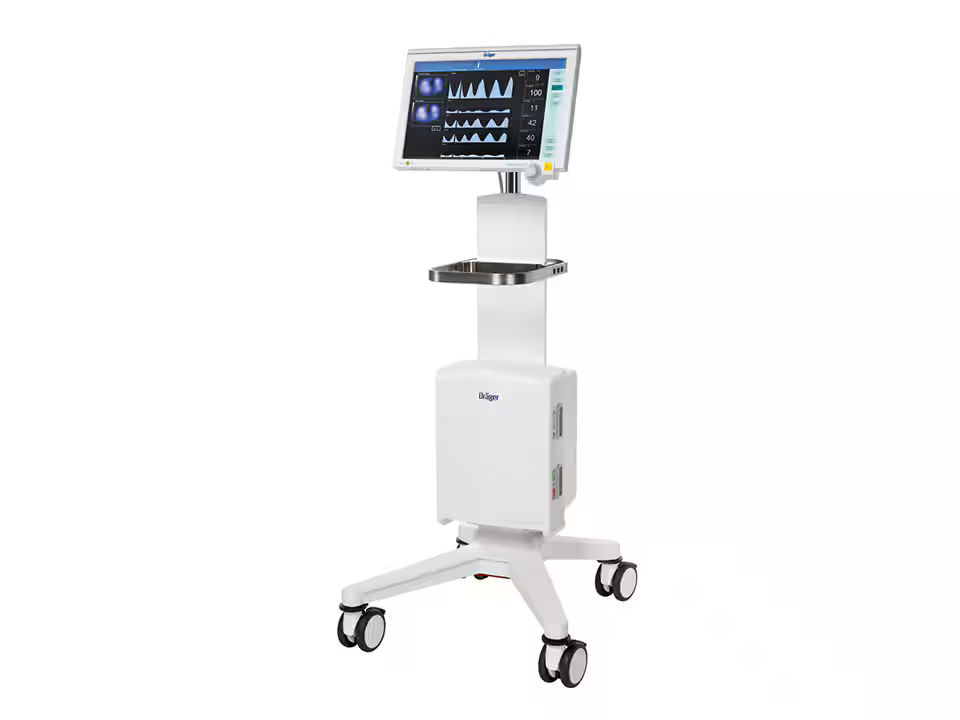
\includegraphics[width=0.4\linewidth]{Figures/draeger-pulmovista-500.png}
%		\hspace{1cm}
%		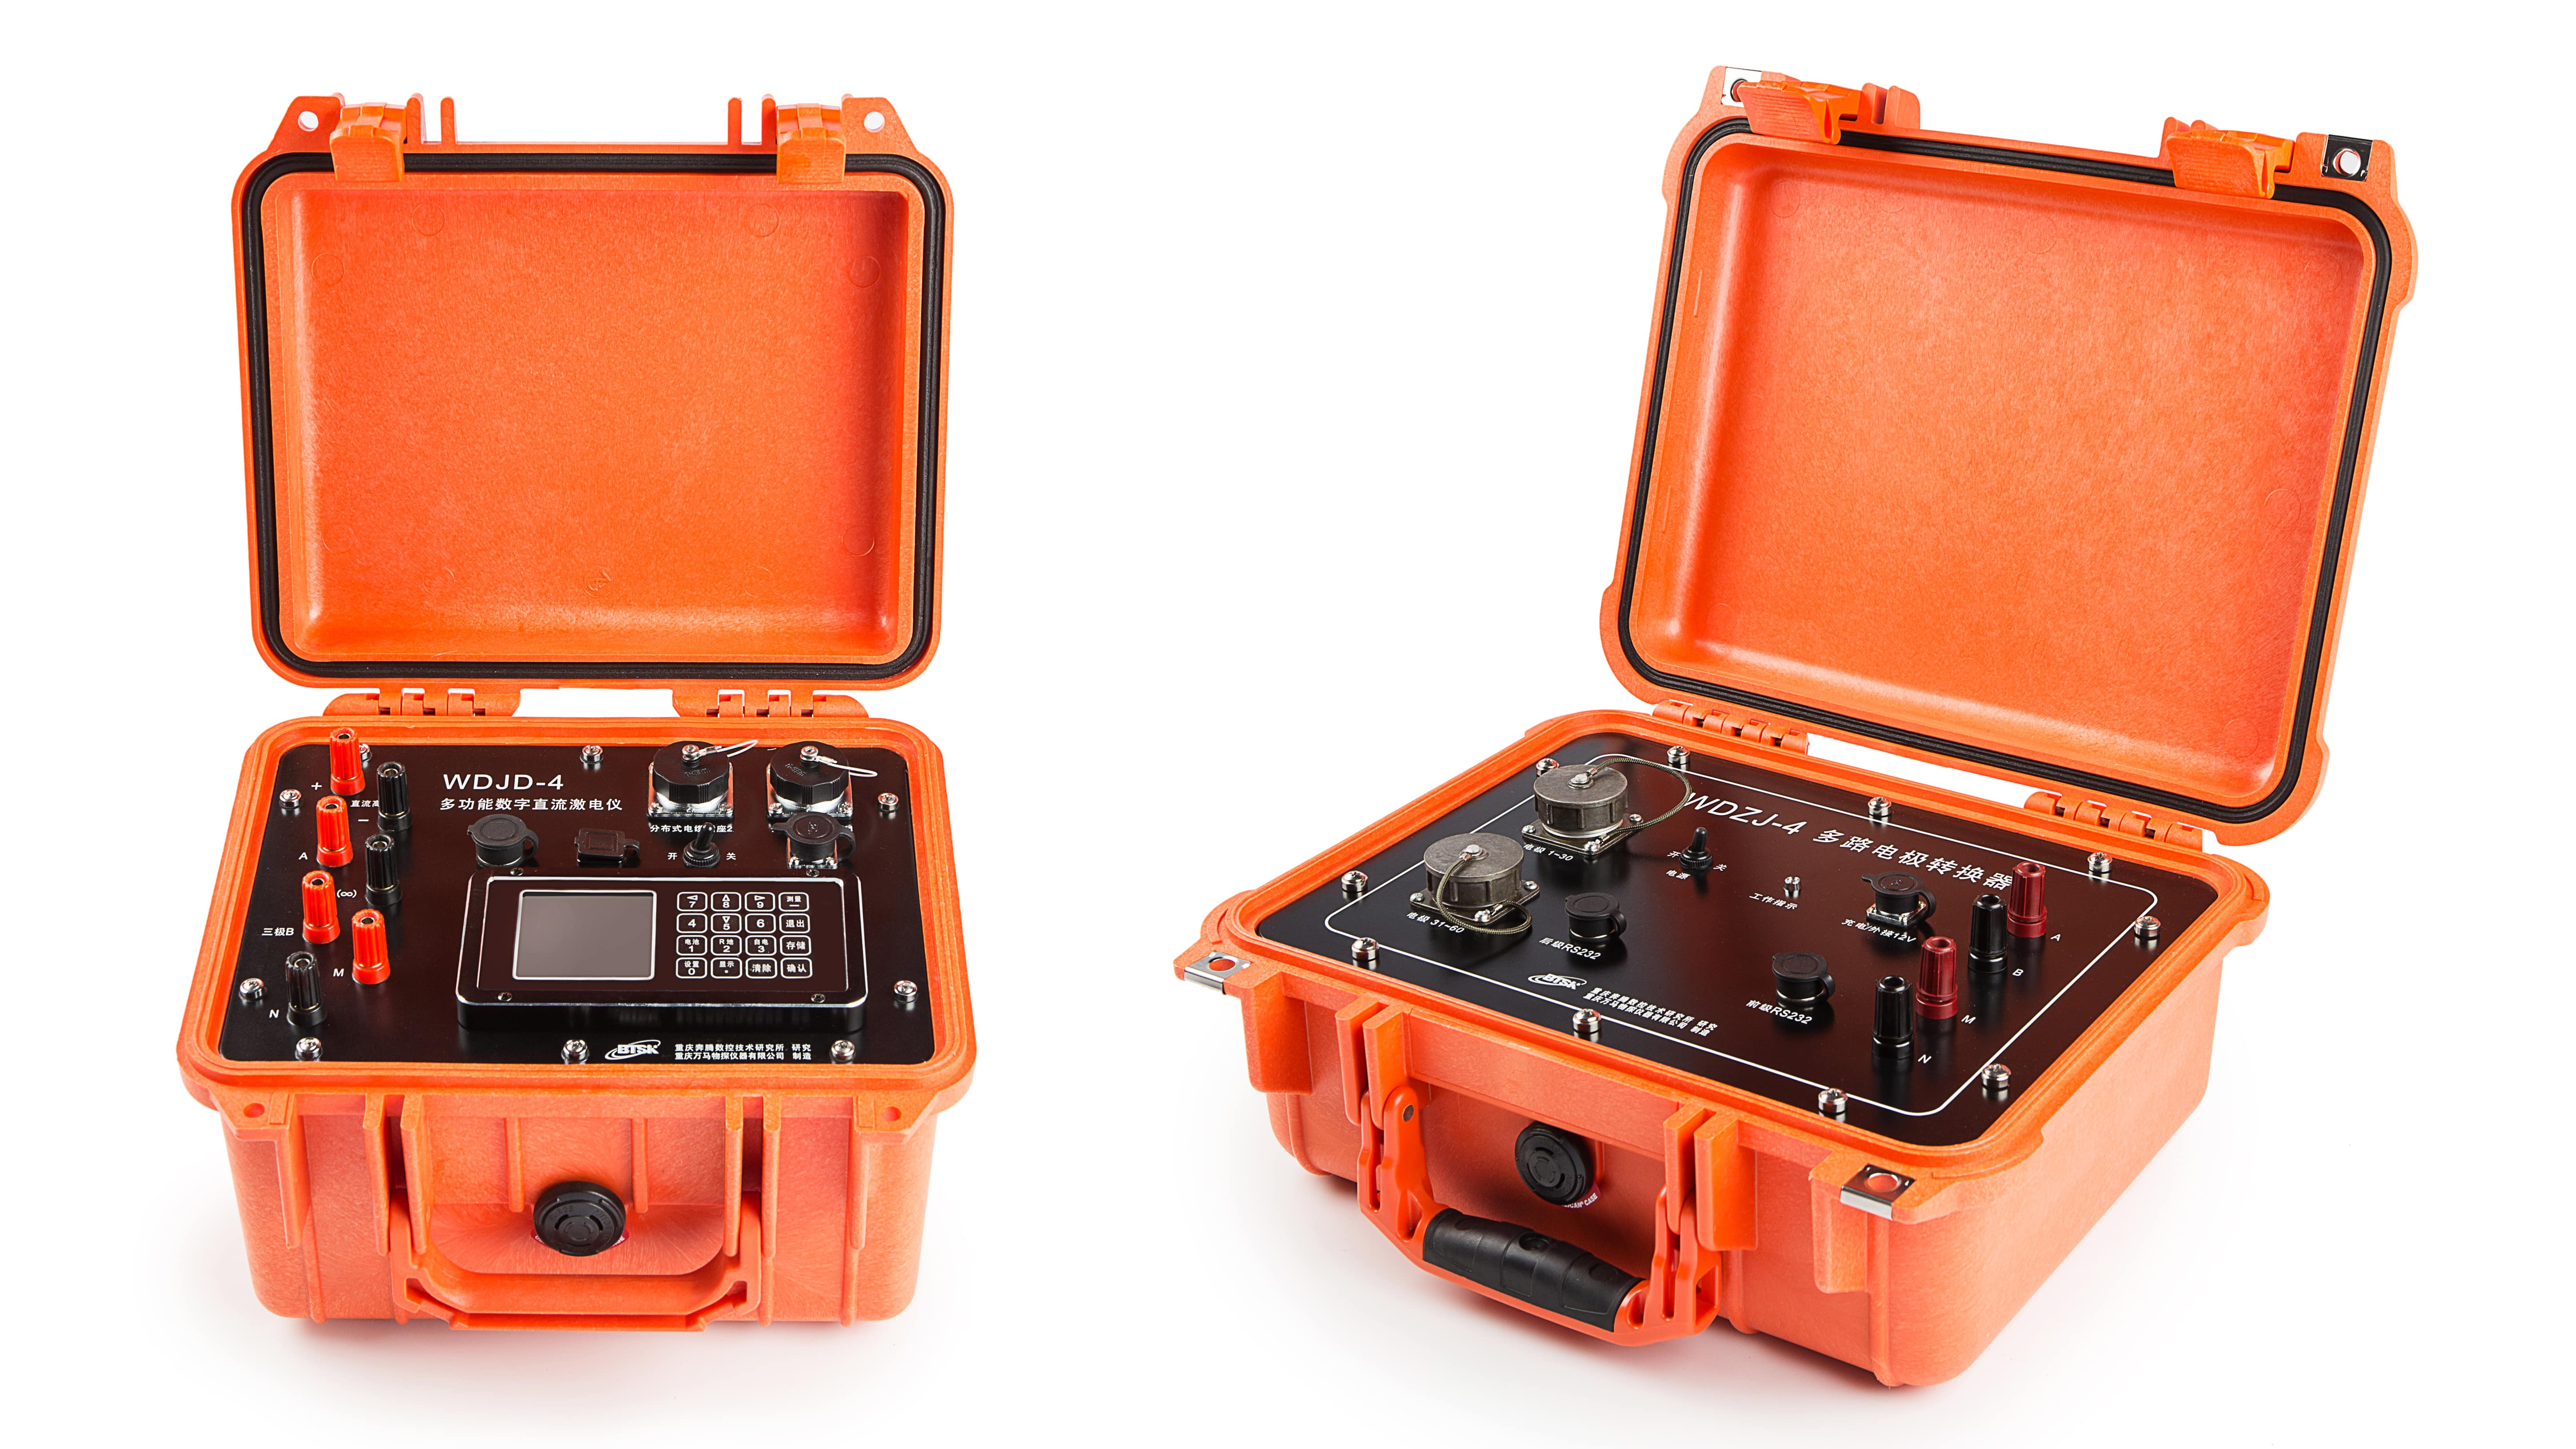
\includegraphics[width=0.4\linewidth]{Figures/ERT_WGMD-4.jpg}
%		\caption{Left: Pulmovista 500 medical thorax EIT machine \cite{Draeger2024}. Right: WGMD-4 ERT geophysical measurement device \cite{WTSGeophysical2024}.}
%		\label{fig:pcb_to_pcba}
%	\end{figure}
In this work the same physics principles used in bio-medical and geophysical sensing are used to map localised compressive loads on a soft piezoresistive material. Pressure mapping is widely used for many applications including sports equipment grip analysis, foot pressure in gait analysis, in production line part alignment, hospital patient bed and chair pressure minimisation, headphone pressure analysis, amongst many others. These applications are useful for increasing quality of life, optimising sporting performance, object detection, and production efficiency optimisation.

A core limiting factor of current technology is the lack of customisability in sensor size, shape, sensing domain material softness, and sensing material composition \cite{Gilanizadehdizaj2022,Rossiter2005,Liang2015,Fu2020}. Most often, pressure sensors are given in a rectangular format because of the arrays of wiring and sensing elements required within the sensing domain. EIT-based pressure mapping sensors are not constrained by wires or complex patterning within the sensing domain area. EIT-based pressure sensors can have a homogeneous sensing domain configured in various shapes.
%	\begin{figure}[H]
%		\centering
%		\includegraphics[width=0.30\linewidth]{Figures/picture showing future application.png} % same sketch style as the literature review sketch. sketch of person with prosthetic arm and with smart soles??
%		\caption{Potential future application of sensor technology}
%		\label{fig:future_app}
%	\end{figure}
To advance the research of this soft pressure mapping platform technology, we require a system that is lost cost, open source, easy to use, portable, and sufficiently flexible to test a range of different sensing domain materials. The system developed in this work is for the research and development of EIT-based pressure mapping sensors. 

The hardware of our system has two key components, a circuit for gathering raw ERT data and a Cartesian force applicator (CFA) machine for characterising an ERT-based pressure mapping sensor. The system characterises the sensor and can be used for validating the spatial, pressure, and temporal performance for different piezoresistive sensor material domains. The CFA allows for repeatable experiments and quantifiable data for different sensor configurations.

\section{Hardware description}
% Describe the hardware, highlighting the customisation rather than the steps of the procedure. Highlight how it differs/which advantage it offers over pre-existing methods. For example, how could this hardware: be compared to other hardware in terms of cost or ease of use, be used in the development of further designs in a particular area, and so on.

Created an EIT-based pressure mapping sensor toolbox that reliably and repetitively allows for EIT-based pressure mapping and quantification of the sensor performance. The overall system is simple to construct and easy to operate and is split into two main parts: the ERT sensor and the CFA device.
\begin{figure}[H]
\centering
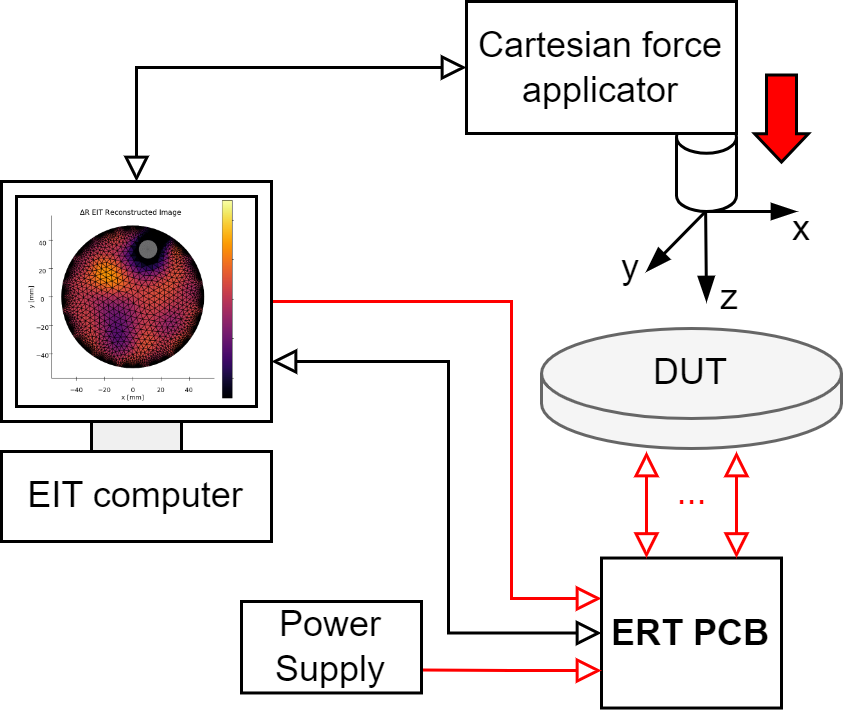
\includegraphics[width=0.4\linewidth]{Figures/ERT_PCB_and_CFA_system_simple.png}
\caption{System architecture of ERT sensor and CFA setup. The large red arrow shows the direction of the force applicator compression onto the sensing domain (DUT) and analogue/power signals are shown with red arrows and digital signals with black arrows.}
\label{fig:ERT_PCB_CFA_archit}
\end{figure}
% ert sensor
The ERT sensor consists of an ERT sensor circuit and the sensing domain under test (DUT). The ERT circuit drives the EIT measurements through the sensing domain soft elastomer composite material. The EIT circuit designed is small (79 x 94 x 12 mm) for potential use in space-constrained mobile applications. 
The system has a programmable current source which can drive up to 50 mA of constant current. The voltage measurement circuit has an ADC resolution of 0.3 $\mu$V, ensuring that the small signals generated by small localised loads can be detected. The sensing domain in this work is a soft piezoresistive composite made from carbon black (CB) powder and silicone rubber with 16 boundary electrodes made from gold pins and copper tape, as seen in Figure \ref{fig:CBSR_samples_examples}.
\begin{figure}[H]
\centering
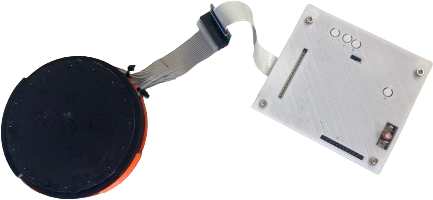
\includegraphics[width=0.50\linewidth]{Figures/ert_pcb_and_DUT.png}
\caption{A soft sensor domain connected to the ERT sensor electronics.}
\label{fig:ert_sensor}
\end{figure}
% cfa
To ensure that the sensor can accurately locate pressure points and their magnitude, the CFA device described in this work is used to apply compressive forces at various locations. The CFA test bed allows for loads within a 220 x 180 mm area.
\begin{figure}[H]
\centering
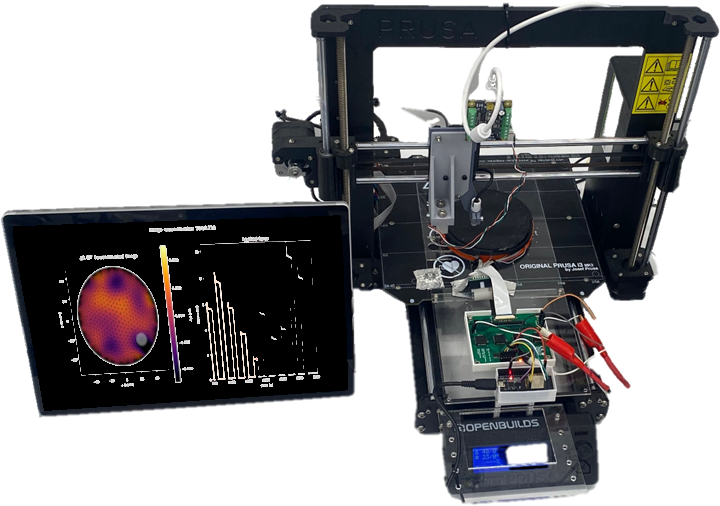
\includegraphics[width=0.5\linewidth]{Figures/cfa_screen_pic.png}
\caption{Cartesian force applicator setup with an ERT circuit and EIT reconstruction computer}
\label{fig:cfa_setup}
\end{figure} 
Previous research groups have developed EIT hardware for pressure mapping sensors \cite{Chen2023,Zhang2017b,Visentin2016,Yoon2017,Sun2020}; however, a complete open-source system including validation hardware has not yet been published. 

To move the field of EIT-based soft pressure mapping forward, there is a need to optimise materials for qualities such as pressure sensitivity, homogeneity, electrode connectivity, and dynamic viscoelastic properties.
This CFA automates the testing process with easily changeable spatio-temporal parameters, such as strain magnitude, strain rate, and strain profile. This system standardises the analysis of the pressure mapping by allowing for the EIT reconstructed resistance images to be compared with stress and strain data form the sensing domain material.

The hope for the hardware and software given in this paper is that it will provide a standardised platform for future researchers to use to further quantify the utility of other sensing materials, and their compare their performance metrics with standard loading test procedures, as done in our previous work \cite{Ellingham2024}.

% > Add 3-5 bulleted points to broadly explain to other researchers how the hardware could be potentially useful to them, for either standard or novel laboratory tasks, inside or outside of the original user community.
\noindent
The ERT sensor and force applicator hardware could be utilised in further research for:
\begin{itemize}
\item 2D piezoresistive material analysis
\item Pressure mapping device characterisation and performance
\begin{itemize}
	\item Spatio-temporal performance
	\item Dynamic stress sensing performance
	\item Piezoresistivity 
\end{itemize}
\item Development for real-world applications
\begin{itemize}
	\item Robotic skin integration
	\item Sports sensing
	\item Prosthetic limbs
\end{itemize}
\end{itemize}

% \section*{\textit{Design files}}
% The  complete  design  files  must  be  either  uploaded  to  an  approved  online  repository,  uploaded  at the  time  of  submission  on  the  online  Editorial  Manager  submission  interface  as  supplementary materials [CAD files, videos,. . . ], or included in the body of the manuscript [e.g.  figures].  The three approved  online  repositories  are  Mendeley  Data,  the  Open  Science  Framework,  and  Zenodo. See repository instructions: https://doi.org/10.5281/zenodo.3346799
% \vskip 0.1 cm
% \noindent
% \textit{\underline{CAD files:} You are encouraged to use free and open source software packages for creating the files. For CAD files, \href{http://www.openscad.org/}{OpenSCAD}, \href{http://www.freecadweb.org/}{FreeCAD}, or \href{https://www.blender.org/}{Blender} are encouraged, but, if these are not available, we accept source files from proprietary CAD packages, such as Autocad or Solidworks, and other drawing packages.} 
% \vskip 0.1 cm
% \noindent
% \textit{\underline{3D printing:} Supplementary files that facilitate digital replication of the devices are encouraged;  for example, STL files for 3D printing components. We recommend uploading CAD files to the \href{http://3Dprint.nih.gov/}{\underline{NIH 3D Print Exchange}} as Custom Labware and then entering the link here.} 
% \vskip 0.1 cm
% \noindent
% \textit{\underline{Electronics:} PCB layouts and other electronics design files can be uploaded to the \href{http://www.ohwr.org/}{\underline{Open Hardware Repository}} or other repositories or as supplementary materials.} 
% \vskip 0.1 cm
% \noindent
% \textit{\underline{Software and firmware:} All software files used in the design and operation of the hardware should be included in the repository. Provide a description of the software and firmware and use extensive comments in the code.}

\section{Design files summary}
% \textit{Complete a separate row for each design file associated with your hardware (including the primary design files). Any empty rows should be deleted.}
The ERT pressure mapping sensor contains a PCB assembly, housing, and wiring. The CFA design includes a selection of off-the-shelf parts as well as custom designed mechanical CAD parts. Table \ref{tab:design_files} contains all of the custom designed parts from the system as well as the software for both the ERT sensor and CFA devices. In this work the mechanical CAD files were generated using Solidworks and the electrcial ECAD files were generated using KiCAD. Programs designed for this system were mainly written in Python and C.

\vskip 0.1cm
\begin{table}[H]
\caption{Summary of all design files.}
\label{tab:design_files}
\tabulinesep=1ex
\begin{tabu} to \linewidth {|X|X[0.65,1]|X[0.35,1]|X[0.8,1]|}
	\hline
	\textbf{Designed parts} & \textbf{File types} & \textbf{Open source license} & \textbf{Location of the file} \\\hline
	%Insert design files  
	\multicolumn{4}{|c|}{\textbf{ERT pressure mapping sensor}} \\\hline
	% ert\_sensor.kicad\_pro & elec CAD part & GPL &        \href{http://doi.org/10.5281/zenodo.11520112}{10.5281/zenodo.11520112} /ERT\_sensor/elec\_CAD/ \\\hline
	PCB design & elec CAD (.kicad\_sch, .kicad\_pcb, .kicad\_pro) & GPL &        \href{http://doi.org/10.5281/zenodo.11520112}{10.5281/zenodo.11520112} /ERT\_sensor/elec\_CAD/ \\\hline
	%			ert\_sensor\_gerber.zip & PCB gerber files & GPL &        \href{http://doi.org/10.5281/zenodo.11520112}{10.5281/zenodo.11520112} /ERT\_sensor/elec\_CAD/ \\\hline
	% ert\_housing\_top.sldprt ert\_housing\_top.stl & mech CAD part & GPL &        \href{http://doi.org/10.5281/zenodo.11520112}{10.5281/zenodo.11520112} /ERT\_sensor/mech\_CAD/ \\\hline
	% ert\_housing\_base.sldprt ert\_housing\_base.stl & mech CAD part & GPL &        \href{http://doi.org/10.5281/zenodo.11520112}{10.5281/zenodo.11520112} /ERT\_sensor/mech\_CAD/ \\\hline
	% domain\_holder\_ptAv2.sldprt domain\_holder\_ptAv2.stl & mech CAD part & GPL &        \href{http://doi.org/10.5281/zenodo.11520112}{10.5281/zenodo.11520112} /ERT\_sensor/mech\_CAD/ \\\hline
	% domain\_holder\_ptCv2.sldprt domain\_holder\_ptCv2.stl & mech CAD part & GPL &        \href{http://doi.org/10.5281/zenodo.11520112}{10.5281/zenodo.11520112} /ERT\_sensor/mech\_CAD/ \\\hline
	3D printed housing & mech CAD parts (.stl, .sldprt) & GPL &        \href{http://doi.org/10.5281/zenodo.11520112}{10.5281/zenodo.11520112} /ERT\_sensor/mech\_CAD/ \\\hline 
	PCB firmware & embedded firmware (.c) & GPL &        \href{http://doi.org/10.5281/zenodo.11520112}{10.5281/zenodo.11520112} /ERT\_sensor/firmware/ \\\hline
	ert\_sensor\_bom.csv & bill of materials & GPL &        \href{http://doi.org/10.5281/zenodo.11520112}{10.5281/zenodo.11520112} /ERT\_sensor/ \\\hline
	
	\multicolumn{4}{|c|}{\textbf{Cartesian force applicator}} \\\hline
	% force\_applicator\_heads & mech CAD parts & GPL &        \href{http://doi.org/10.5281/zenodo.11520112}{10.5281/zenodo.11520112} /CFA/mech\_CAD/ \\\hline
	% PINDA\_adapter.sldprt PINDA\_adapter.stl & mech CAD part & GPL &        \href{http://doi.org/10.5281/zenodo.11520112}{10.5281/zenodo.11520112} /CFA/mech\_CAD/ \\\hline
	% loadcell\_bracket.sldprt loadcell\_bracket.stl & mech CAD part & GPL &        \href{http://doi.org/10.5281/zenodo.11520112}{10.5281/zenodo.11520112} /CFA/mech\_CAD/ \\\hline
	% ert\_sample\_tray.dxf & mech CAD part & GPL &        \href{http://doi.org/10.5281/zenodo.11520112}{10.5281/zenodo.11520112} /CFA/mech\_CAD/ \\\hline
	% ert\_ckt\_tray.dxf & mech CAD part & GPL &        \href{http://doi.org/10.5281/zenodo.11520112}{10.5281/zenodo.11520112} /CFA/mech\_CAD/ \\\hline
	% ert\_ckt\_tray\_bearing.sldprt ert\_ckt\_tray\_bearing.stl & mech CAD part & GPL &        \href{http://doi.org/10.5281/zenodo.11520112}{10.5281/zenodo.11520112} /CFA/mech\_CAD/ \\\hline
	% phidget\_bridge\_mount.sldprt phidget\_bridge\_mount.stl & mech CAD part & GPL &        \href{http://doi.org/10.5281/zenodo.11520112}{10.5281/zenodo.11520112} /CFA/mech\_CAD/ \\\hline
	Fabricated parts & mech CAD parts (.stl, .sldprt) & GPL &        \href{http://doi.org/10.5281/zenodo.11520112}{10.5281/zenodo.11520112} /CFA/mech\_CAD/ \\\hline 
	Testing software & data capture/ processing (.py) & GPL &        \href{http://doi.org/10.5281/zenodo.11520112}{10.5281/zenodo.11520112} /CFA/software/ \\\hline
	%			ertpcb\_cfa\_reader.py & data capture software & GPL &        \href{http://doi.org/10.5281/zenodo.11520112}{10.5281/zenodo.11520112} /CFA/software/ \\\hline
	%			default\_eit\_recon.py & data processing software & GPL &        \href{http://doi.org/10.5281/zenodo.11520112}{10.5281/zenodo.11520112} /CFA/software/ \\\hline
	cfa\_bom.csv & bill of materials & GPL &        \href{http://doi.org/10.5281/zenodo.11520112}{10.5281/zenodo.11520112} /CFA/ \\\hline
\end{tabu}
\end{table}

% For each design file listed in the summary above, include a short description of the file below (one or two sentences)
\subsection{ERT pressure mapping sensor file descriptions}
% \textbf{ert\_sensor.kicad pro}
% \\ \\
\textbf{PCB design} - KiCAD project files including the electrical schematics and PCB layout for the ERT sensor circuit.
\\ \\
%	\textbf{ert\_sensor\_gerber.zip} - PCB gerber and drill files for fabrication.
%	\\ \\
% \textbf{ert\_housing\_top.sldprt ert\_housing\_top.stl} - 3D printed PLA lid for ERT sensor enclosure.
% \\ \\
% \textbf{ert\_housing\_base.sldprt ert\_housing\_base.stl} - 3D printed PLA box for ERT sensor enclosure.
% \\ \\
% \textbf{domain\_holder\_ptAv2.sldprt domain\_holder\_ptAv2.stl} - 3D printed PLA holder base for ERT sensor domain material.
% \\ \\
% \textbf{domain\_holder\_ptCv2.sldprt domain\_holder\_ptCv2.stl}- 3D printed PLA holder top for ERT sensor domain material.
% \\ \\
\textbf{3D printed housing} - CAD files for 3D printed sensor enclosure and a sensor domain holder example.
\\ \\
\textbf{PCB firmware} - Firmware for the ERT data capture driving the electrode drive pattern through multiplexer switching. The data captured is then streamed via serial to a seperate reconstruction processor.
\\ \\
\textbf{ert\_sensor\_bom.csv} - Bill of materials for all parts and components in the ERT PCBA.
\\ \\

\subsection{Cartesian force applicator file descriptions}

%	\textbf{force\_applicator\_heads} - A library of 3D printed PLA force applicator heads for applying a known surface shapes to the domain.
%	\\ \\
% \textbf{PINDA\_adapter.sldprt PINDA\_adapter.stl} - A 3D printed PLA structure for holding the MK3s inductive sensor for print bed height calibration.
% \\ \\
% \textbf{loadcell\_bracket.sldprt loadcell\_bracket.stl} - A 3D printed PLA bracket to mount the loadcell onto the 3D printer frame.
% \\ \\
% \textbf{ert\_sample\_tray.dxf} - A laser cut 4 mm thick acrylic sheet of plastic to align the CFA with the domain material. 
% \\ \\
% \textbf{ert\_ckt\_tray.dxf} - A laser cut 4 mm thick acrylic sheet of plastic to hold the ERT electronics. 
% \\ \\
% \textbf{ert\_ckt\_tray\_bearing.sldprt ert\_ckt\_tray\_bearing.stl} - A simple bearing surface for the sensor tray to slide on.
% \\ \\
% \textbf{phidget\_bridge\_mount.sldprt phidget\_bridge\_mount.stl} - A 3D printed PLA mount for the loadcell electronics.
% \\ \\
\textbf{Fabricated parts} - CAD for 3d printed and laser cut parts  for the modification of the 3D printer platform into a CFA.
\\ \\
\textbf{Testing software} - Software for simultaneous force, position, and ERT data acquisition and processing.
\\ \\
%	\textbf{ertpcb\_cfa\_reader.py} - Software for simultaneous force, position, and ERT data acquisition.
%	\\ \\
%	\textbf{default\_eit\_recon.py} - Software for for the default reconstruction of a circular sensing domain containing 16 electrodes using the serial data files generated from \textit{ertpcb\_cfa\_reader.py}.
% remove this software?
%	\\ \\
\textbf{cfa\_bom.csv} - Bill of materials for all parts in the CFA system apart from the ERT sensor electronics.



\section{Bill of materials}
% > For material type, select from: Metal, semi-conductor, ceramic, polymer, biomaterial, organic, inorganic, composite, nanomaterial, semiconductor, non-specific, or other  
Please refer to the two detailed bills of materials (BOMs) given in Table \ref{tab:design_files}.



\section{Build instructions}
%Provide detailed, step by step instructions for the construction of the reported hardware include all necessary information for reproducing the submitted hardware. Example of reference designator usage (U9:PDM1-S12-S5-S) (REF:MPN)
% > Explain and, when possible, characterize design decisions. Including design alternatives if they exist. 
% > Use visual instructions such as schematics, images, and videos. 
% > Clearly reference design files and component parts described in the Design File Summary and Bill of Materials. 
% > Highlight potential safety concerns that may arise
The build is separated into two parts. The first being the assembly of the ERT sensor electronics and housing. The second being the build of the Cartesian force applicator. Text within square brackets refer to the part reference designators (e.g. U1 for the ESP32 module) in the BOMs.


\subsection{ERT Sensor}
% grab gerber files send to PCB manufacturer. Place all SMD components. Place all THT components. Don't place jumpers until circuit has been tested. Copy and paste circuit test procedure. Place in housing for mounting on Prusa.
The manufacturing process of the PCB involves first sending the PCB gerber files to a PCB manufacturer. This work used JLC PCB with their default parameters for a 4 layer PCB.

Next populate the PCBs with the SMD parts given in the BOM and place in a reflow oven. First complete the rear side then the top side to ensure components stick. Once all SMD parts have been firmly soldered, solder all of the THT components. Finally attach the jumpers for the desired power mode, explained in Section \ref{sec:Operating modes}.
\begin{figure}[H]
\centering
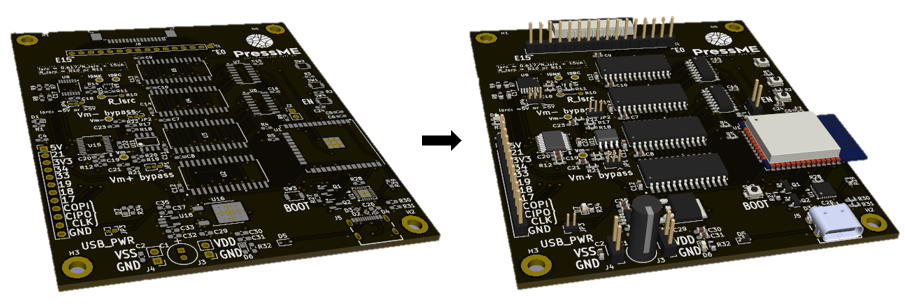
\includegraphics[width=0.8\linewidth]{Figures/HV_ERT_sensor_PCB_unpop2pop.png}
\caption{ERT PCB [PCB1] before and after electrical component population.}
\label{fig:pcb_to_pcba}
\end{figure}
To ensure simple protection against electrical shorts and low-level ingress protection (equivalent to IP20) 3D print an enclosure in PLA using the STL files given in the BOM, \textit{ert\_housing\_top.stl} [PR1] and \textit{ert\_housing\_base.stl} [PR2]. There are 4 threaded inserts [HW2] to mount the PCB securely in the 3D printed enclosure using four M3 14 mm bolts [HW1].

Attach the 16 way ribbon connector [W1] to the ERT electrodes. In this example there is a ribbon to IDC connector interface board [J8], which then connects to a custom built electrode pin to domain interface [DUT1, DUT2, PR3, PR4]. This electrode interface will vary based on the required sensing domain.
\begin{figure}[H]
\centering
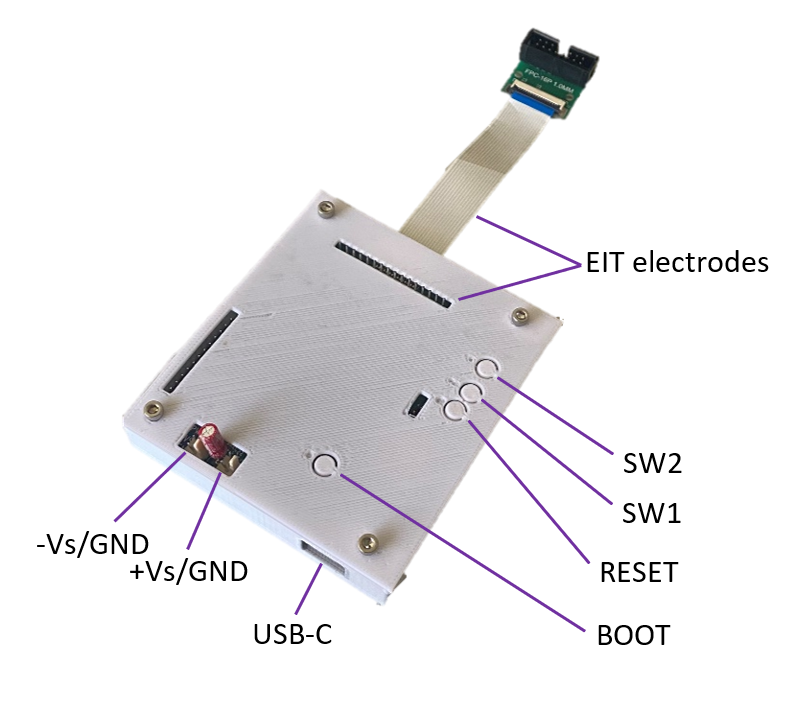
\includegraphics[width=0.6\linewidth]{Figures/ERT_PCB_assembled_in_housing_labelled.png}
\caption{ERT sensor PCBA mounted in enclosure and attached electrode harness showing buttons and the main electrical connections.}
\label{fig:ert_sensor_in_housing}
\end{figure}
The sensor device shown in Figure \ref{fig:ert_sensor_in_housing} shows all of the connections and buttons necessary for the programming and operation of the sensor, as well as two optional buttons SW1 and SW2 for any other desired functions.

\subsection{Sensing Domain}
\label{sec:Sensing Domain}
% basically copy and paste from other papers

%	>> delete this whole section? If not, change to imperative tense?

As a reference the method for fabricating a specific sensing domain is given in this section. The sensing domain used was a carbon black (CB) nanoparticle silicone rubber composite.

With the material requirements of a low Shore hardness of 5A - 25A, similar to that of human skin and muscle tissue \cite{Silvera-Tawil2015, Chatzistergos2022}, low viscoelasticity, high yield strength, low resistivity, high strain gauge factor, and non-toxic. Other sensor domain materials may be used for the sensor, such as soft conductive particle composites, conductive polymers, and hydrogels \cite{Giffney2017,Duan2014,Chen2023}.

Researchers fabricating their own sensing domain for use with this system should follow three key requirements, 
\begin{enumerate}
\item The size of the sensing domain must fit within a 220 x 180 x 160 mm volume (X$\times$Y$\times$Z) on the CFA test bed. 
\item The bulk modulus of the domain material must be chosen such that the required loads applied to the domain must not exceed 100 N.
\item The inter-electrode resistance, $R_{int}$, must be low enough to not saturate the current source, $I_{src}$, given a power supply voltage, $V_s$, as shown in Equation \ref{eqn:r_int},
\end{enumerate}
\begin{equation}
R_{int} < \alpha \frac{V_s}{I_{src}}
\label{eqn:r_int}
\end{equation}
Where $R_{int}$ is the resistance values between every configuration of the current drive electrodes during an EIT capture cycle and $\alpha$ is the factor of safety for any electrode movement or incidental increase of $R_{int}$ during experimentation.

The domain under test (DUT) used in this work was a composite comprised of XC 72R carbon black (CB) nanoparticles (Cabot, Alpharetta, USA) [DUT5] of 50 nm average diameter, dispersed in a two part Dragon Skin 10 NV silicone rubber (SR) matrix (SmoothOn, Macungie, USA) [DUT6]. The weight percentage (wt\%) of CB to liquid silicone rubber which resulted in near optimal piezoresistive characteristics was found to be between 8 - 10\%. To ensure homogeneous CB particle dispersion and mitigate air bubble formation an ARV-310 vacuum planetary mixer (Thinky, Tokyo, Japan) was used to mix the CB particles through the liquid silicone matrix. Upon completion of mixing, the uncured composite was poured into the circular sheet domain mould. The curing of the composite was controlled by heating the newly-mixed material in the mould at 80$\degree$C for 90 min. The domain samples used in this work and previous work \cite{Ellingham2022, Ellingham2024} had a diameter of 100 mm as shown in Figure \ref{fig:CBSR_samples_examples}. 

\begin{figure}[H]
\centering
% 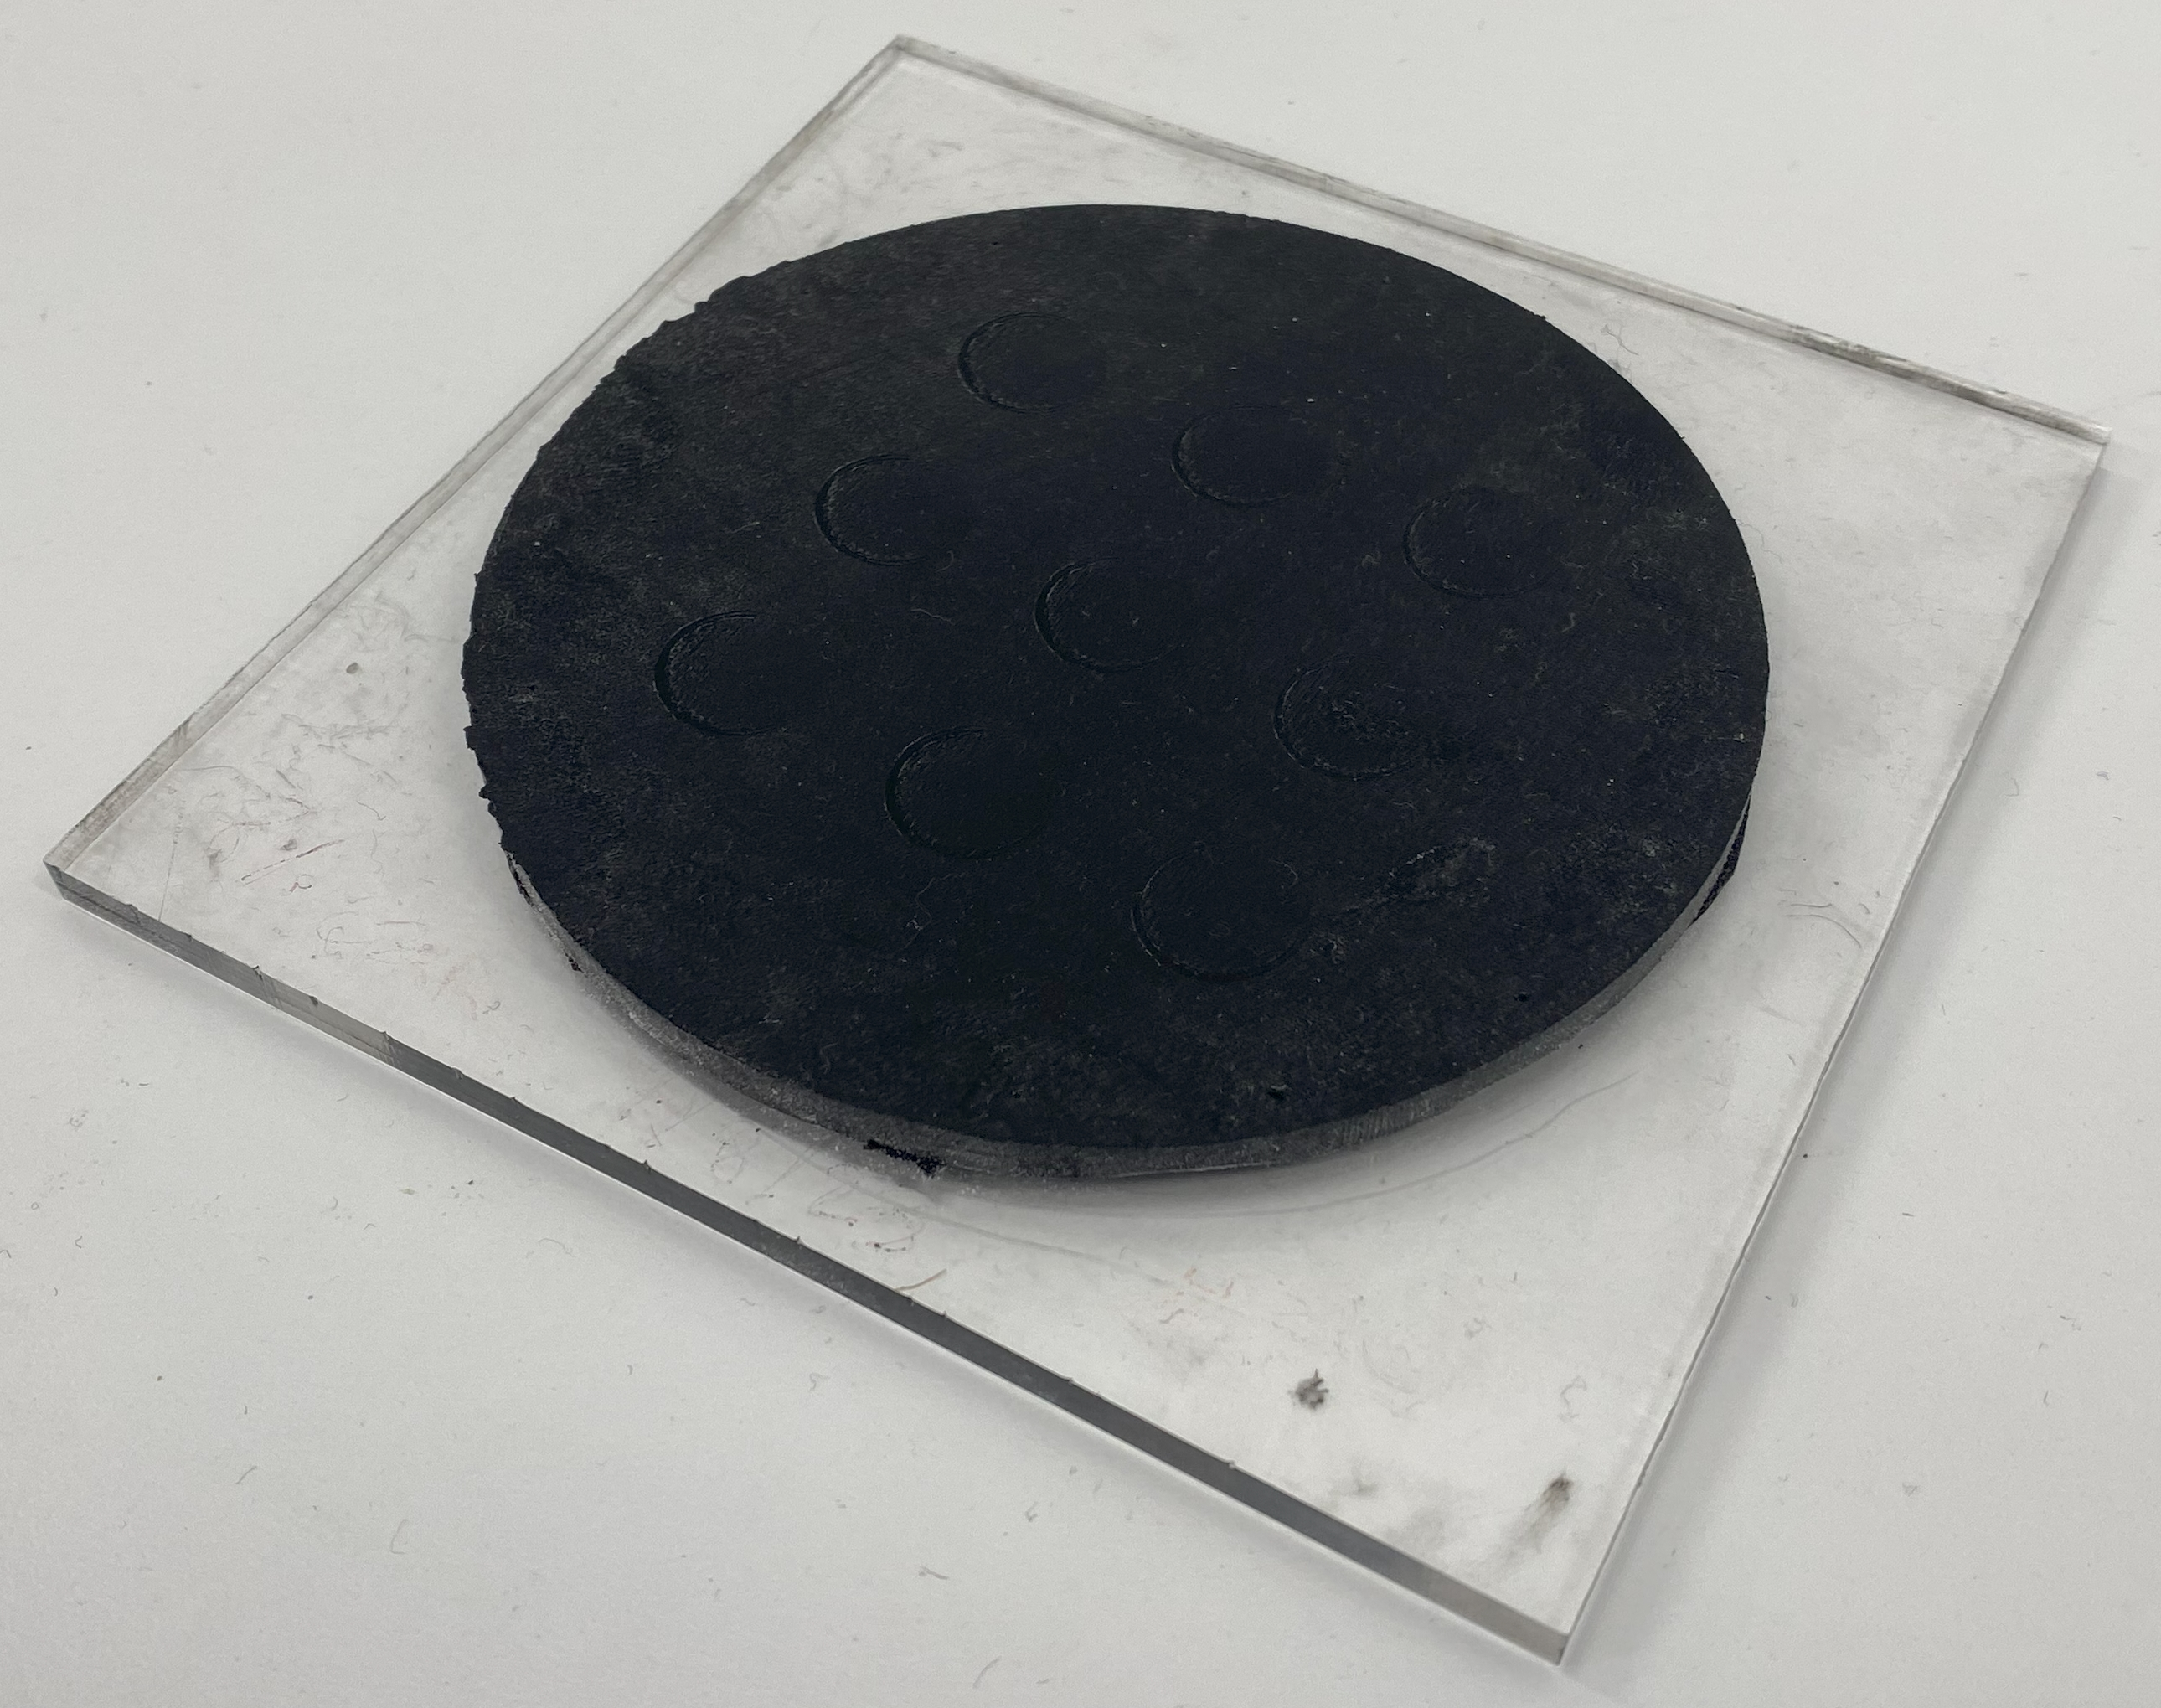
\includegraphics[width=0.295\linewidth]{Figures/CBSR_DUT_sample.jpg}
% 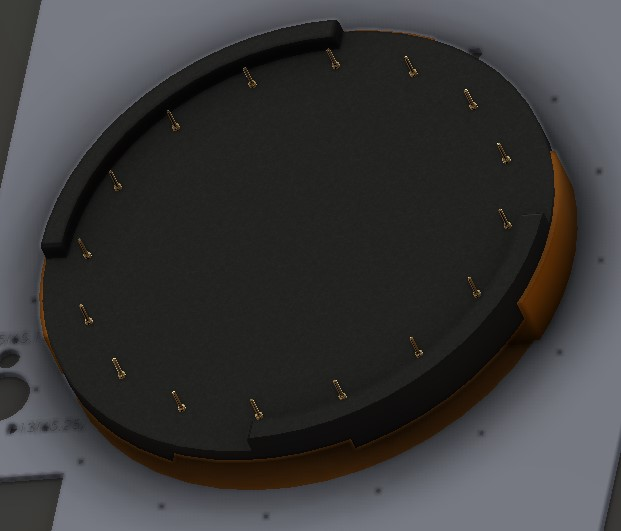
\includegraphics[width=0.275\linewidth]{Figures/ERT_sensing_domain_holder2.jpg}
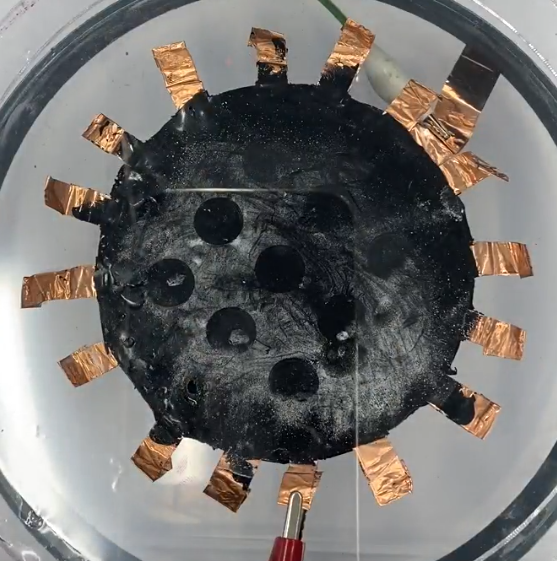
\includegraphics[width=0.3\linewidth]{Figures/DEA-EIT-sample_0.5mm_100mm.png}
\hspace{2cm}
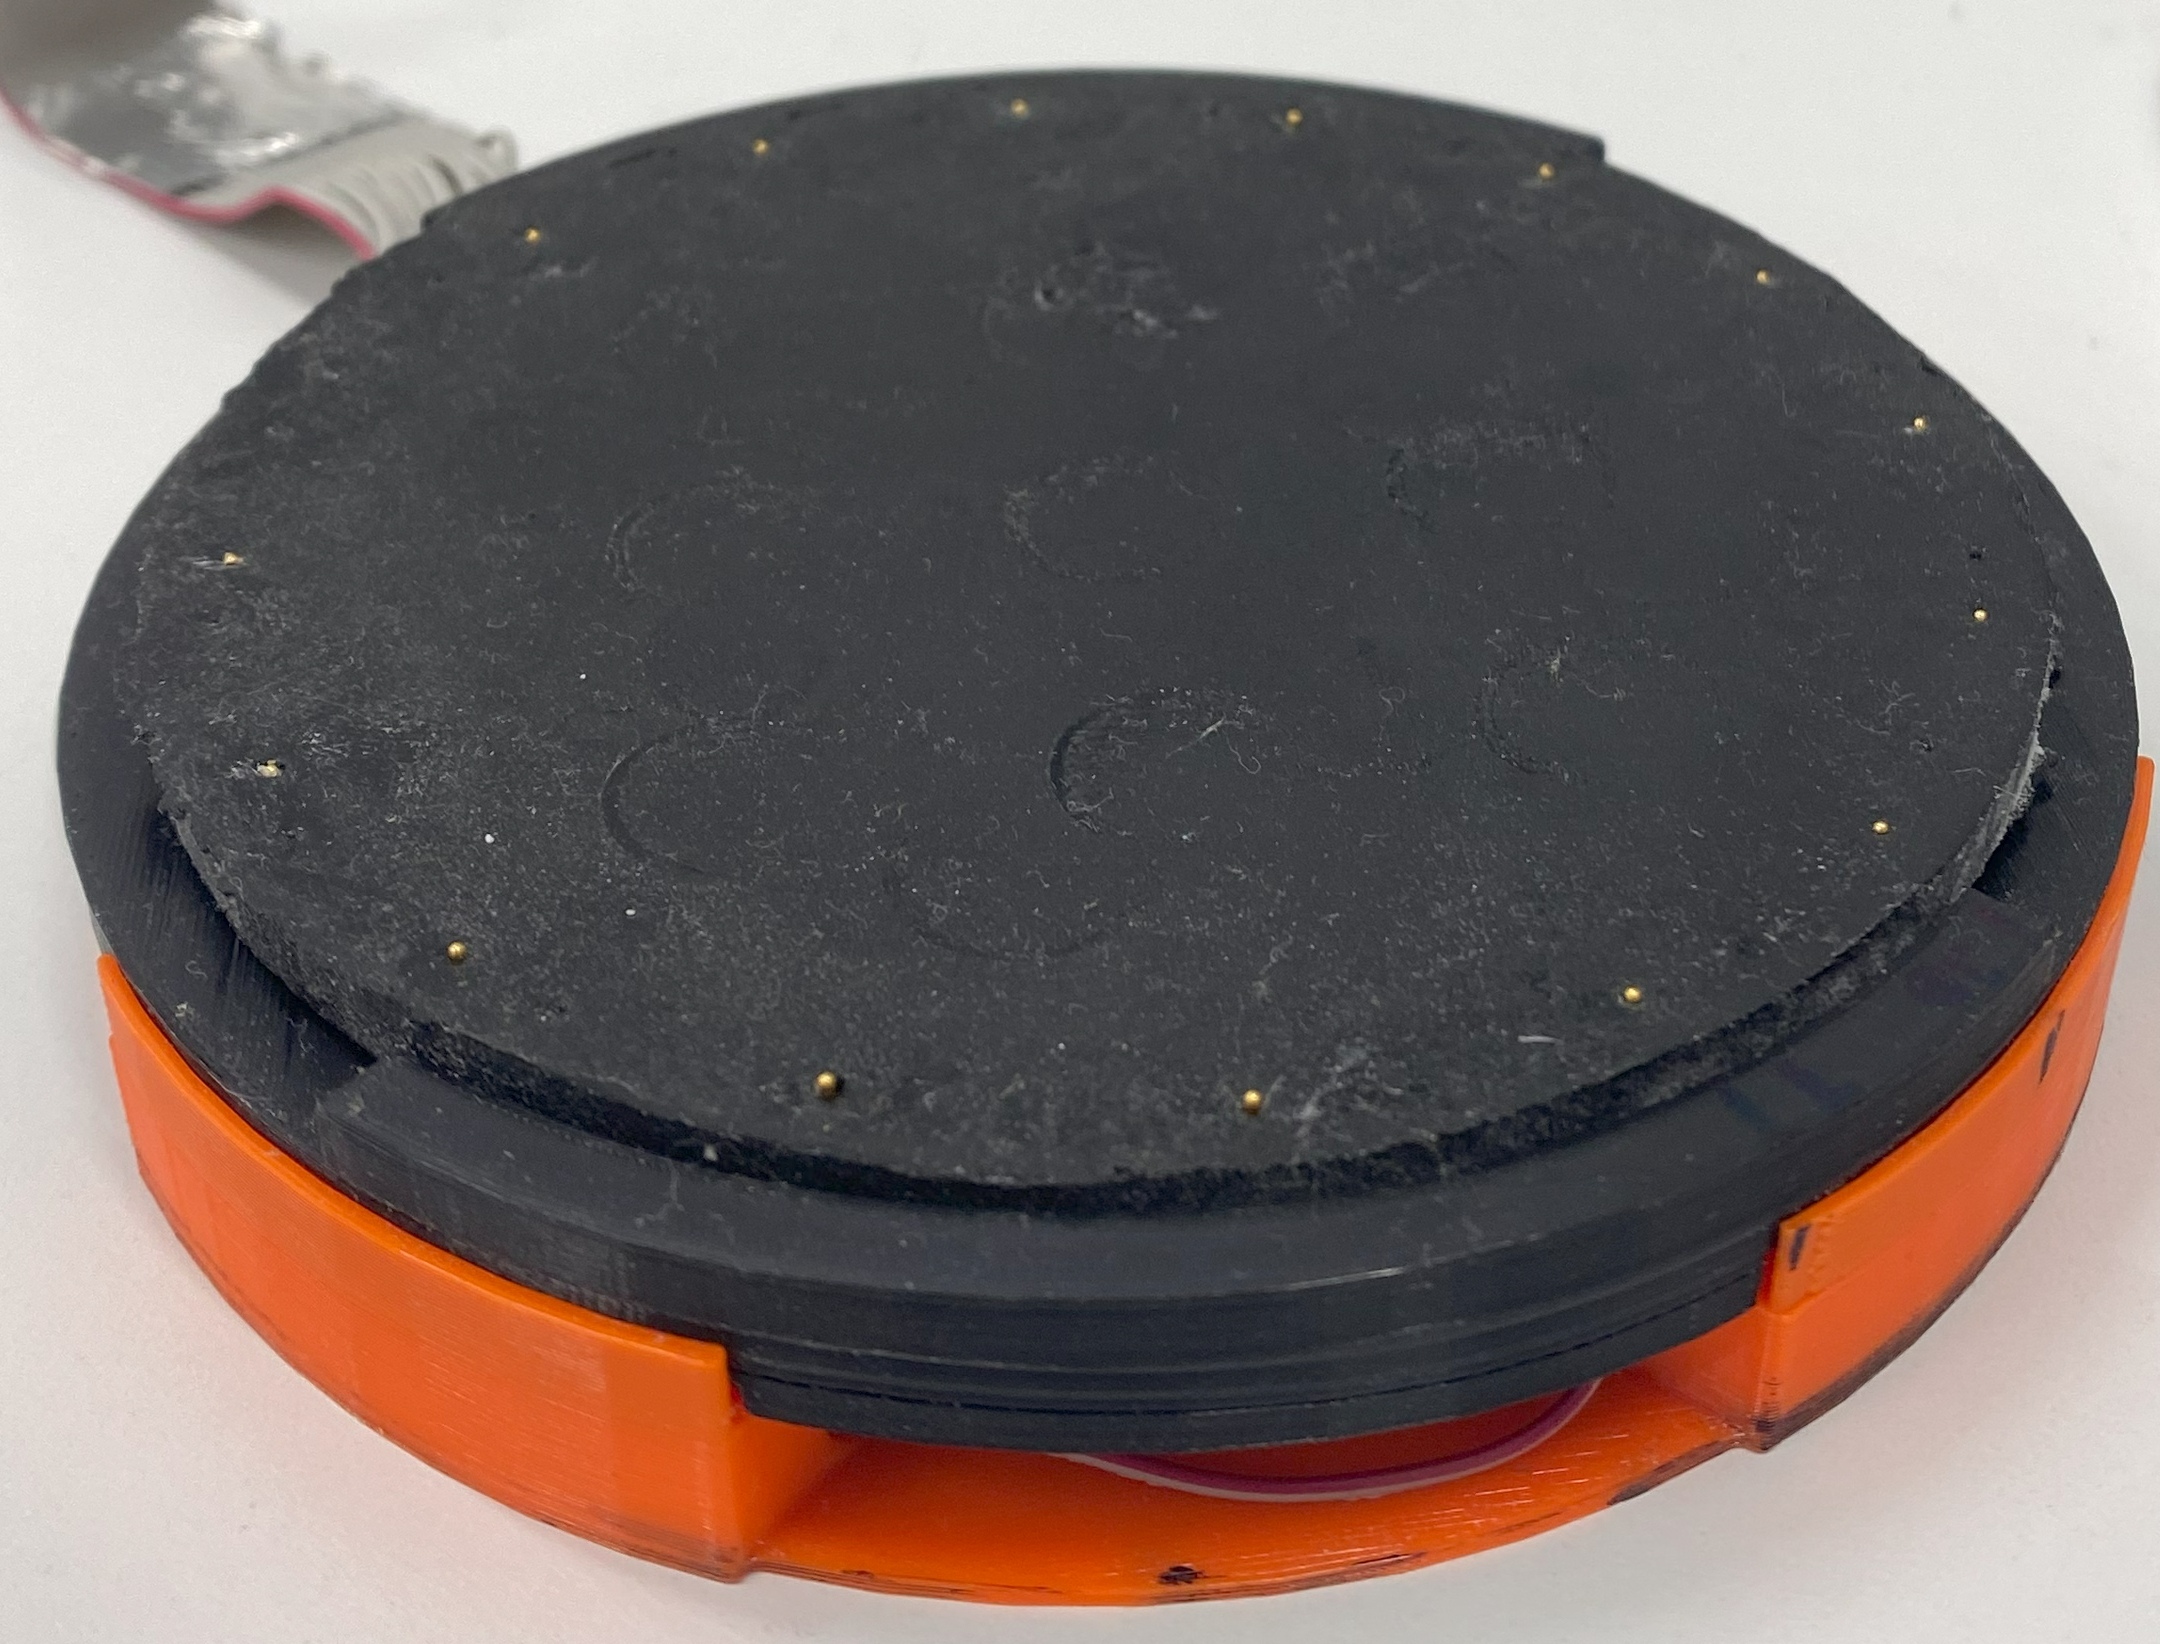
\includegraphics[width=0.4\linewidth]{Figures/CBSR_DUT_w_electrodes_sample.jpg}
\caption{Left: An example of a CBSR sample with copper tape electrodes integrated with a dielectric elastomer actuator setup \cite{Ellingham2024a}. Right: Example of a CBSR sensing domain with gold pin electrodes penetrating material surface around the sensing region boundary.}
\label{fig:CBSR_samples_examples}
\end{figure}


\subsection{Cartesian force applicator}
% Dismantle prusa printhead and trick thermistor. Mount loadcell, loadcell bridge, sensor tray, etc. Prepare sensing region surface...
To test the spatial and force resolution of the ERT pressure mapping device, the CFA was designed using a Prusa MK3s 3D printer to provide a stable platform. First a functional Prusa MK3s 3D printer was acquired with its printing capabilities tested on several standard demo PLA prints to ensure the print head can move with the expected resolution in the X, Y, and Z directions. Standard benchmark tests and tuning for the printing platform can be found  \href{https://blog.prusa3d.com/does-your-freshly-assembled-original-prusa-i3-mk3-print-as-the-best-it-can_29445/}{here} and \href{https://help.prusa3d.com/category/print-quality-troubleshooting_225}{here} \cite{Stritesky2019, Prusa2024}.

\begin{figure}[H]
\centering
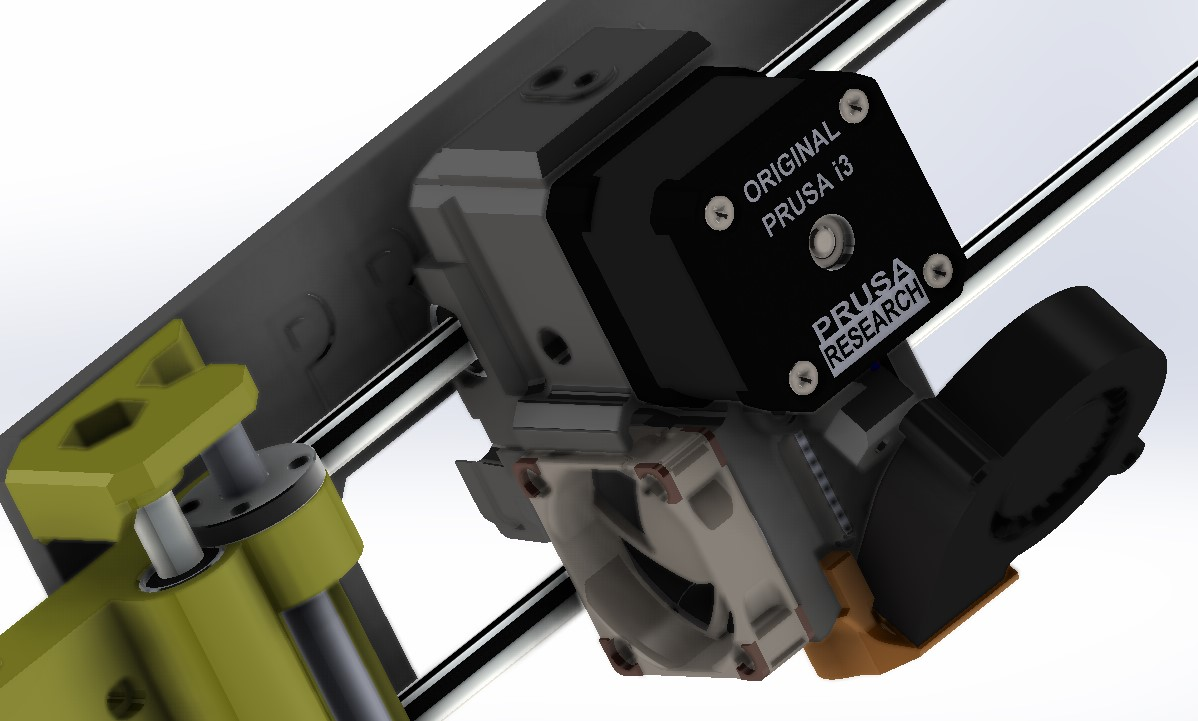
\includegraphics[width=0.4\linewidth]{Figures/og_MK3s_print_head.jpg}
\hspace{1cm}
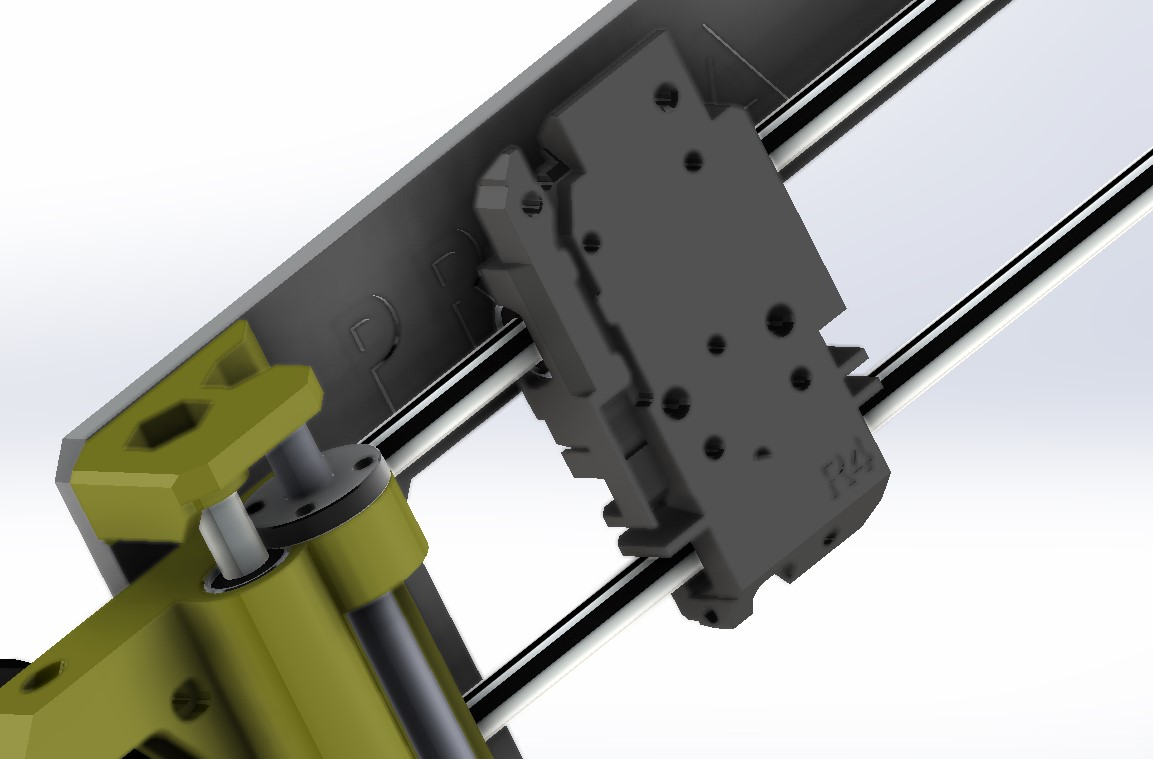
\includegraphics[width=0.4\linewidth]{Figures/dismantled_MK3s_print_head.jpg}
% 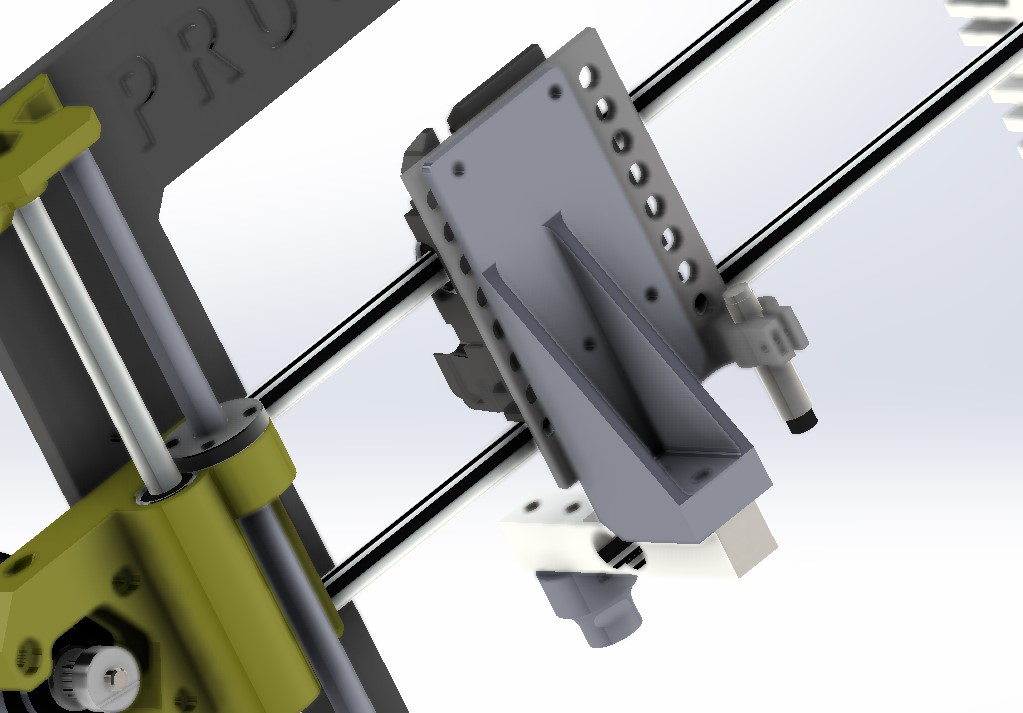
\includegraphics[width=0.32\linewidth]{Figures/modded_MK3s_print_head.jpg}
\caption{MK3s print head. Left: Original print head assembly. Right: Dismantled print head assembly \cite{Kayne2019}.}
\label{fig:mk3s_head_old_raw}
\end{figure}

Next the print head of the MK3s was dismantled, as shown in Figure \ref{fig:mk3s_head_old_raw}, leaving a flat surface to attach first the PINDA adapter [PR8] and the loadcell bracket [PR9], as shown in Figure \ref{fig:mk3s_head_new}. Use M3 bolts to attach the loadcell bracket and PINDA adapter to the dismantled print head surface. See read the printer \href{https://help.prusa3d.com/guide/5-e-axis-assembly_169235#170079}{assembly manual} for more detail on the part assembly\cite{Prusa2023}. Bolt the TAL220 10 kg loadcell [E3] onto the loadcell bracket using M5 bolts [HW4]. Bolt the force applicator head [PR5-7, HW5] onto the other end of the loadcell using M4 bolts [HW3]. A range of force applicator heads shapes and sizes have been created to test the resolution of the sensor. 
\begin{figure}[H]
\centering
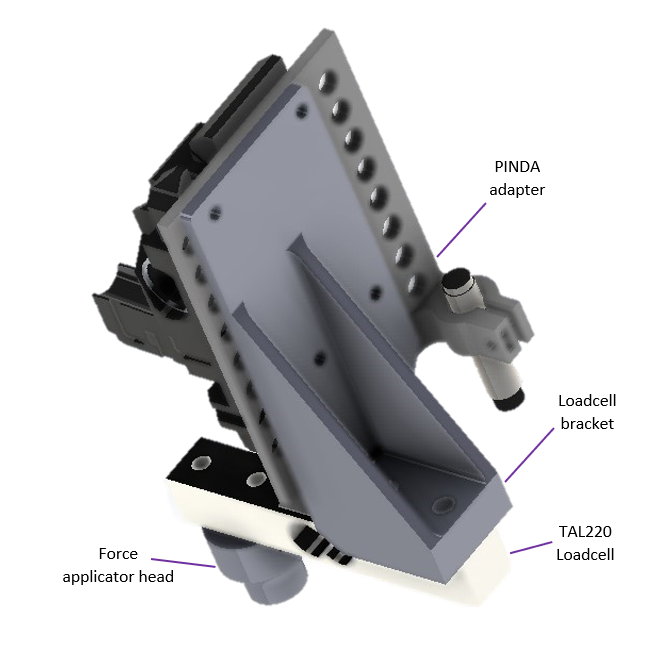
\includegraphics[width=0.5\linewidth]{Figures/modded_MK3s_print_head_clean_labelled.png}
\caption{Force applicator head assembly.}
\label{fig:mk3s_head_new}
\end{figure}
With the thermistor from the original printhead no longer required, a trimpot [RV1] is attached to the thermistor port on the printer's \href{https://help.prusa3d.com/guide/8-electronics-assembly_174100#175539}{control circuit PCBA}\cite{Prusa2023a}. While the 3D printer is turned on, the trimpot is manually adjusted until room temperature is reached on the 3D printer display to avoid any future under/over temperature errors.

The print bed of the MK3s 3D printer is removed and replaced with a mount tray [LC1] for the sensing domain. The ERT tray bearing part [PR10] mounted and bolted [HW6] onto the frame of the MK3s as shown in Figure \ref{fig:mk3s_new_trays}. The ERT sensor tray [LC2] and the sensing domain mount tray are fixed together onto the print bed with two M3 bolts [HW6] clamping the trays to the edge of the print bed.

\begin{figure}[H]
\centering
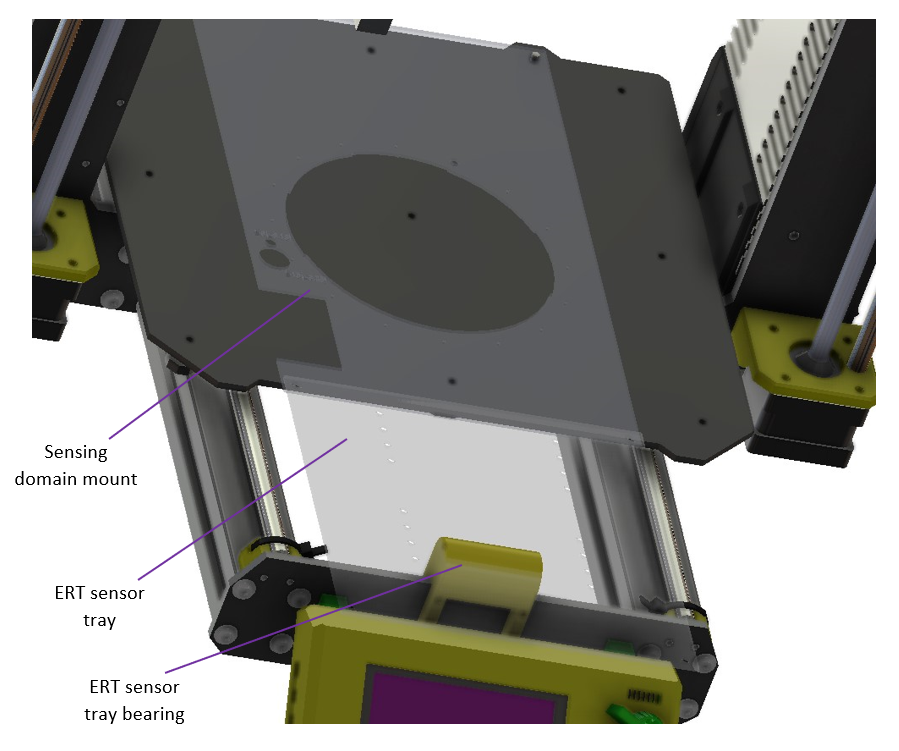
\includegraphics[width=0.6\linewidth]{Figures/cfa_trays_assm_labelled.png}
\caption{MK3s with original print bed tray removed and the ERT sensor trays added.}
\label{fig:mk3s_new_trays}
\end{figure}

The firmware version used in this work was MK3s 3.9.0. Later versions may be compatible. Other 3D printer platforms with a similar gcode command set and a similar core firmware such as the \href{https://marlinfw.org/}{Marlin firmware} may also be used as a CFA. However, minor configuration changes in this work's software and hardware may be required.


\section{Design Decisions}
% validate the main design decision contributing to the performance and novelty of the system.
This section outlines and justifies some of the important design decisions made for both the ERT sensor and the CFA device.
\begin{figure}[H]
\centering
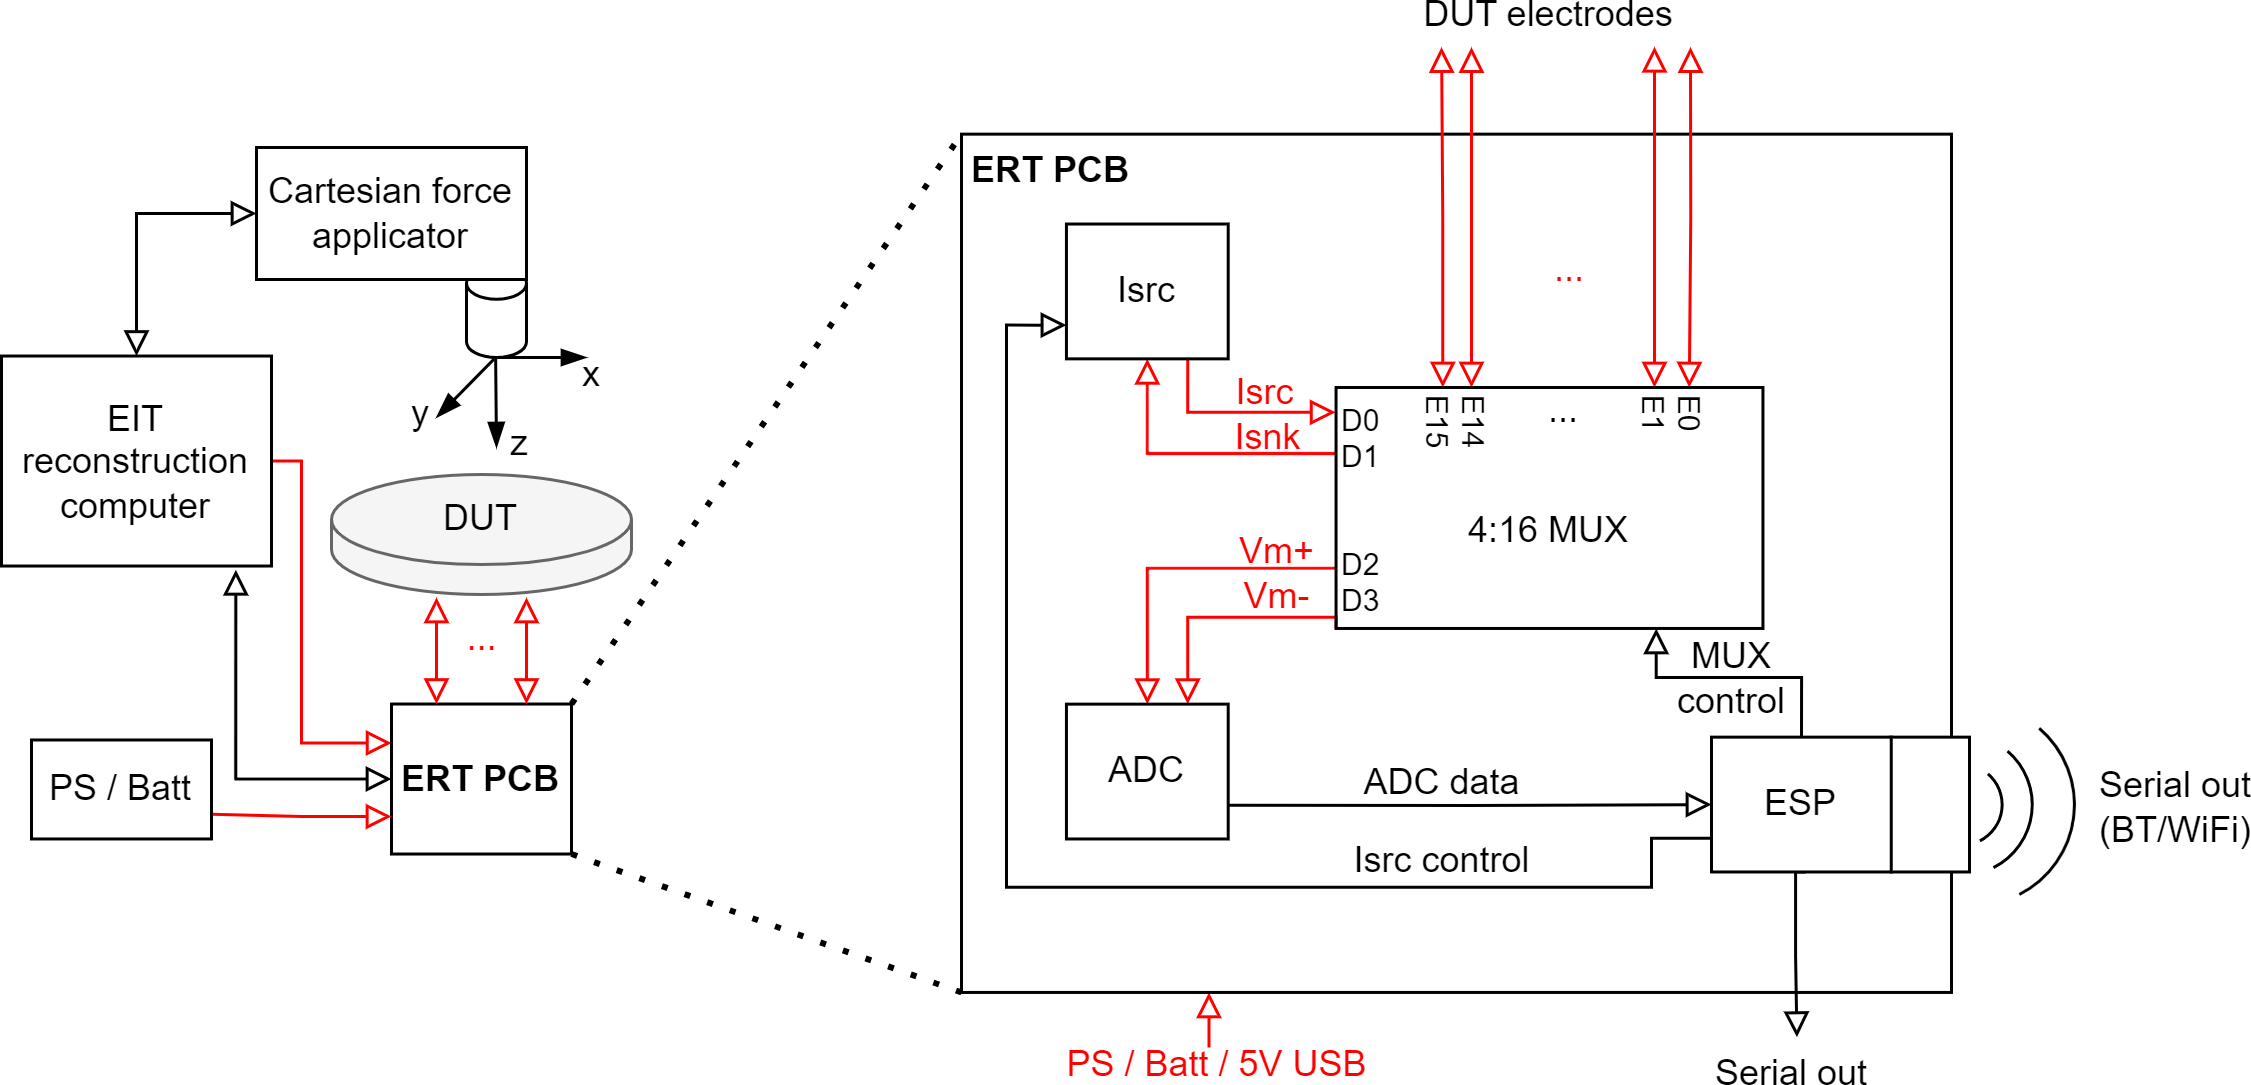
\includegraphics[width=0.9\linewidth]{Figures/ERT_PCB_and_CFA_system.png}
\caption{System architecture of ERT sensor and CFA setup (left) and the key internal electrical signals of the ERT circuit (right). With analogue/power signals shown with red arrows and digital signals with black arrows.}
\label{fig:ERT_PCB_CFA_archit}
\end{figure}


\subsection{EIT cycle and load sequence}
While a sequence of compressive loads are applied by the CFA to the sensing domain, concurrently the ERT sensor circuit gathers data for EIT reconstruction. This cyclic EIT data capture process follows a specific sequence, 
\begin{figure}[H]
\centering
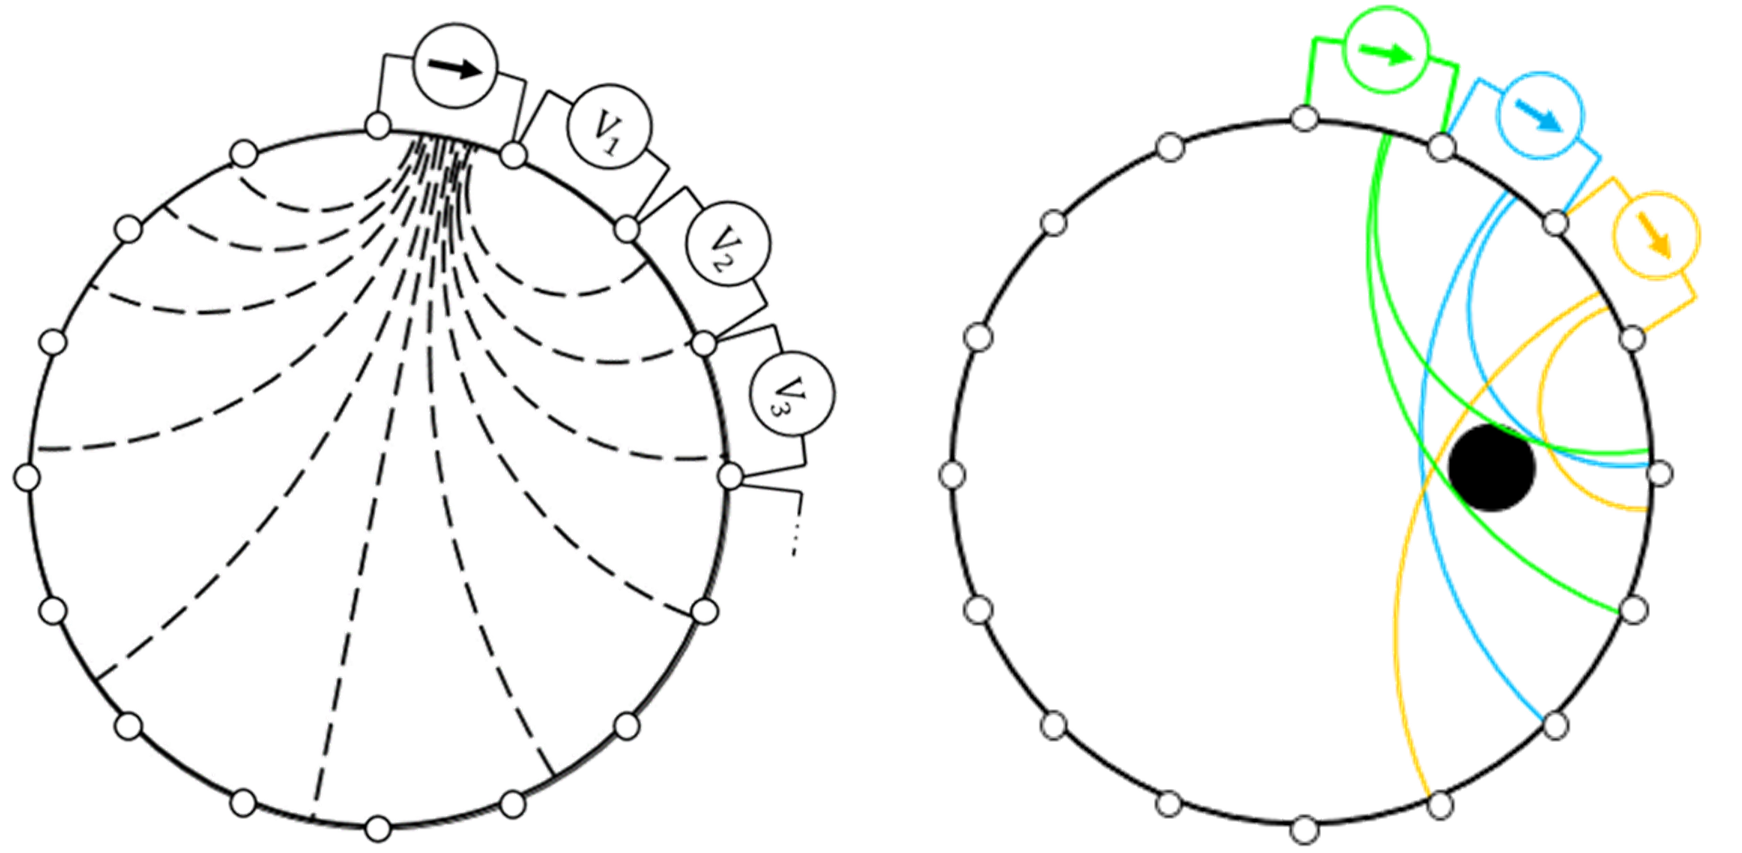
\includegraphics[width=0.7\linewidth]{Figures/eit_sequence.png}
\caption{EIT adjacent drive pattern sequence.}
\label{fig:ERT_PCB_CFA_archit}
\end{figure}
\begin{enumerate}
\item A constant current is applied at adjacent electrode positions $E_i$ and $E_{i+1}$, these electrode positions are selected with the `MUX control' line.
\item Sequentially 16 adjacent electrode voltage measurements are completed next, again the electrode positions are selected with the `MUX control' line.
\item Each raw voltage measurement is transmitted through `serial out' to an `EIT reconstruction computer'.
\item The next current injection electrode position is selected, i.e. i = i + 1. Once all 16 current injection positions are completed, 256 voltages are measured giving enough data for one reconstruction frame. This is repeated for the duration of the experiment.
\end{enumerate}
Multiplexing of the voltage measurements was chosen instead of the alternative option of simultaneous voltage measurement, to maintain a low-cost circuit. The simultaneous voltage measurement solution involves 16 separate ADCs, one for each electrode. A DC current source was chosen instead of the AC alternative because the sensing domains do not show significant changes in reactance during loading events.


\subsection{Small signal measurement}
% important because precision measurements required for EIT.
The range of voltages required for recreating minute changes in resistances of a sensing domain spans several orders of magnitudes. Therefore a high dynamic range, high resolution, low-noise voltage measurement system is required to capture this data.

% Include resistor mesh network validation for range of expected votlages?
To evaluate the performance of the system with a standardised testing domain a resistor mesh network was created. The mesh network was created to validate the expected resolution required for generating EIT reconstructions \cite{Ellingham2022} for a variety of different resistances and resistance changes. The resistor mesh network provided a standardised platform with known resistor values and tolerances for the comparison a real and simulated resistor mesh network. The resistor mesh network was chosen to provide a range EIT voltage data comparable to that of the real CBSR composite material.

A script was created to form a square resistor mesh network of various dimensions and various background resistance values. PySpice circuit simulator \cite{PySpice2021} was used to run a zero noise simulation on the system to show the expected difference in raw ERT voltage data between a homogeneous resistor mesh and a resistor mesh with an anomalous blob as shown in Figure \ref{fig:vdiff_res_mesh}. The maximum and minimum $\Delta V_{read}$ values shown in Figure \ref{fig:vdiff_res_mesh} and 94.994 mV and 53 $\mu$V respectively.
\begin{figure}[H]
\centering
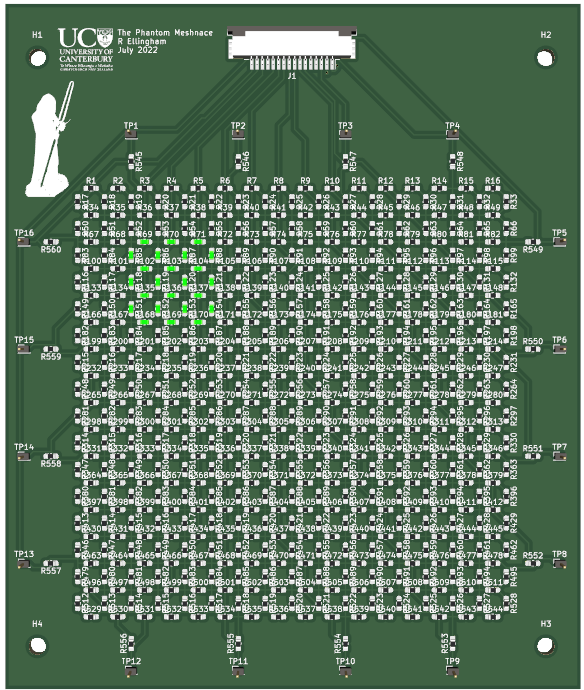
\includegraphics[width=0.3\linewidth]{Figures/res_mesh_pcb.png}
\hspace{1cm}
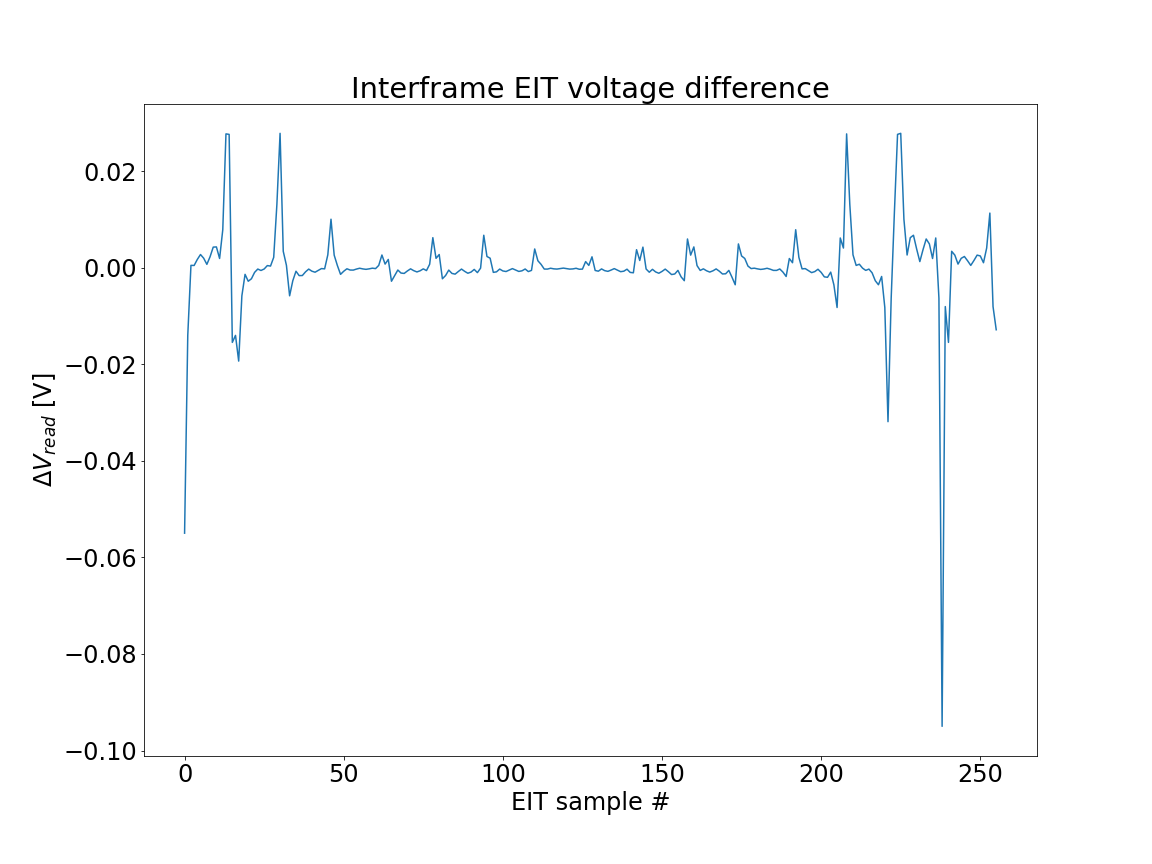
\includegraphics[width=0.5\linewidth]{Figures/EIT_Vdiff_res_mesh_2k2bg_3k3anom.png} % TODO: change this to a dotted plot as these values shouldn't be linked.
\caption{Left: A resistor mesh network for validating the ERT circuit, with the anomaly shown highlighted in green. Right: The difference between EIT raw voltage data from a homogeneous square 2.2 k$\Omega$ resistor mesh domain and the same domain with a 3.3 k$\Omega$ resistor mesh anomaly.}
\label{fig:vdiff_res_mesh}
\end{figure}

It is non-trivial to determine the exact resolution required for an EIT based pressure mapping sensor voltage measurements as it depends on the inherent noise of the domain, the force resolution required, the expected external noise, the drive current, the EIT reconstruction algorithm used, amongst other factors. This work uses a 24 bit ADC [U12] so that given an ideal noiseless representative domain the minimum voltage data shown in Figure \ref{fig:vdiff_res_mesh} will be an order of magnitude larger than the resolution of the ADC.


\subsection{Signal generation}
% quantify and discuss importance of the isrc circuit..
The current source can drive a current, $I_{src}$ between 15 $\mu$A and 50 mA and can be set as a programmable or fixed current source value. The $I_{src}$ value can be altered by changing the $R_{Isrc}$ [R7 or R8] value as shown in Equation \ref{eqn:isrc}.
\begin{equation}
I_{src} = \frac{0.617}{R_{Isrc}} + 15 \space \mu A
\label{eqn:isrc}
\end{equation}
If a fixed current source is desired for the ERT circuit $R_{Isrc}$ sets the current source value based on Equation \ref{eqn:isrc}. If the circuit is configured as a programmable current source, the digital potentiometer [U9] controlling the $R_{Isrc}$ value will a multiple of 39 $\Omega$ up to a maximum of 10 k$\Omega$ or a high impedance state. The possible programmable current source values are given in the \verb|isrc_lookup.xlsx| file in the repository. If the resistivity of the domain is too high the current source supply will saturate to Vs. Ensure the domain resistivity is sufficiently low for this current source saturation not to occur within its expected range of use. 
A sufficiently high current value must pass through the domain to ensure low noise readings throughout the boundary electrodes on the domain. This noise predominantly occurs due to electrostatic effects in sensing domains. To ensure this current can be driven for the sensor domain configuration given in this work, a supply voltage, $\pm V_s$, of $\pm$20 V should be used.


\subsection{Signal conditioning}
% quantify and discuss importance of the opamp circuit and opamp selection. input bias current, Voffset etc...
When using the recommended supply voltage of $\pm$20 V, an attenuation stage is required for the input into the ADC. This is done with an operational amplifier (opamp) voltage buffer-divider-buffer circuit as shown in Figure \ref{fig:opamp_ckt}. When using a single ended 5 V supply to drive the current source this opamp circuit can be bypassed using the jumpers shown in Figure \ref{fig:ert_pcb_pinout_mode} as the attenuation is not required and the offset and noise due to the opamp circuit can be avoided. However due to a lack of a negative $Vss$, the multiplexer channel resistance will be degraded as exemplified in Figure \ref{fig:mux_r_on}.
\begin{figure}[H]
\centering
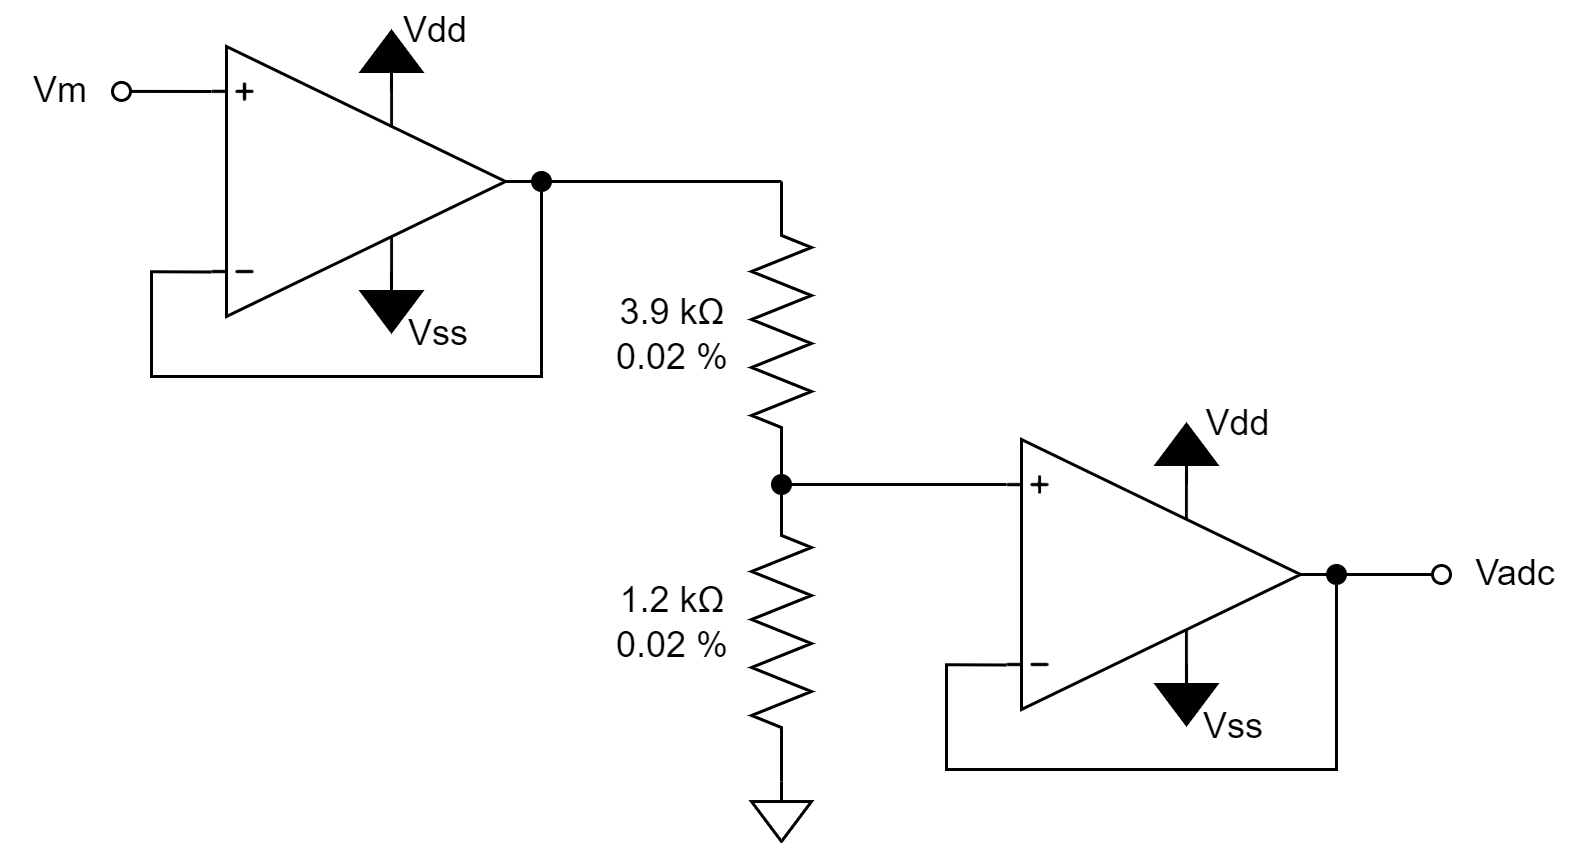
\includegraphics[width=0.5\linewidth]{Figures/opamp_ckt_ert_pcb.png}
\caption{Measurement attenuation circuit}
\label{fig:opamp_ckt}
\end{figure}
To allow larger current signals to be driven through the domain a maximum voltage driving the current source of 20 V is used with an attenuation circuit consisting of two voltage buffers and a voltage divider. The attenuation circuit steps down the voltage with a nominal gain of 0.24 $\pm$ 3\%. The attenuation circuit is duplicated for both differential ADC inputs. This circuit is highly sensitive to any noise, DC offset, or component variation. To combat the sensitivity of this circuit the opamps used [U10, U11] have a low input bias current, and low input DC offset voltage, the resistors used have a low tolerance of $\pm$0.02\%.
\begin{figure}[H]
\centering
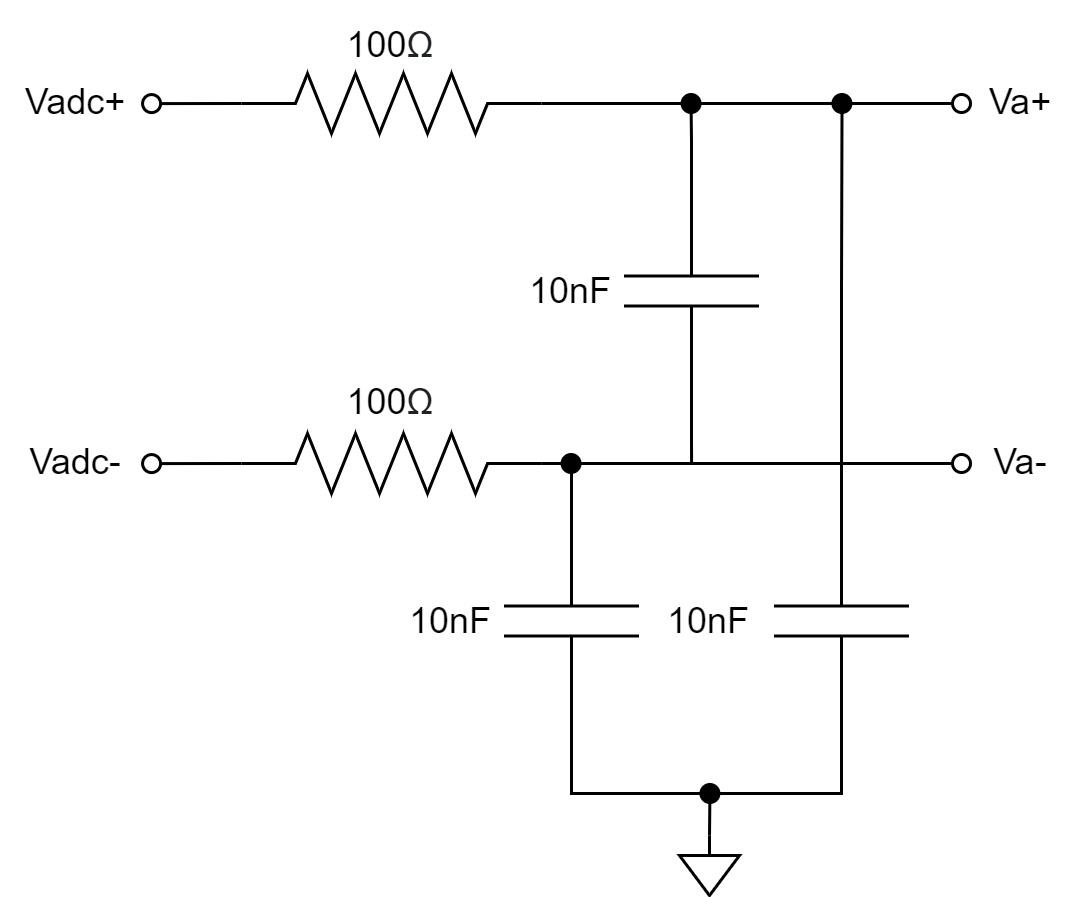
\includegraphics[width=0.4\linewidth]{Figures/adc_filter_ckt.png}
\caption{Passive low-pass filter circuit}
\label{fig:adc_filter_ckt}
\end{figure}
A passive low-pass filter has been placed between the opamp circuit and the ADC input to attenuate ADC input noise. The cutoff frequency for this filter has been set to a value of, 1 MHz allowing for sufficient settling time for the maximum potential ADC sample rate of 512 kSPS.


\subsection{Switching circuit}
% plot the Ron characteristic again VD for a set VDD/VSS??
A 4:16 multiplexing circuit allows for a range of EIT switching drive patterns for ERT data acquisition. Previous research has shown the trade-offs with different EIT drive patterns \cite{Tawil2011, Russo2017, Xu2008}. A multiplexer with a low drain-source on-resistance characteristic for smaller drain voltages has been chosen as the majority of the voltage readings being read through the multiplexer will be nearer to zero than $\pm$Vs.
\begin{figure}[H]
\centering
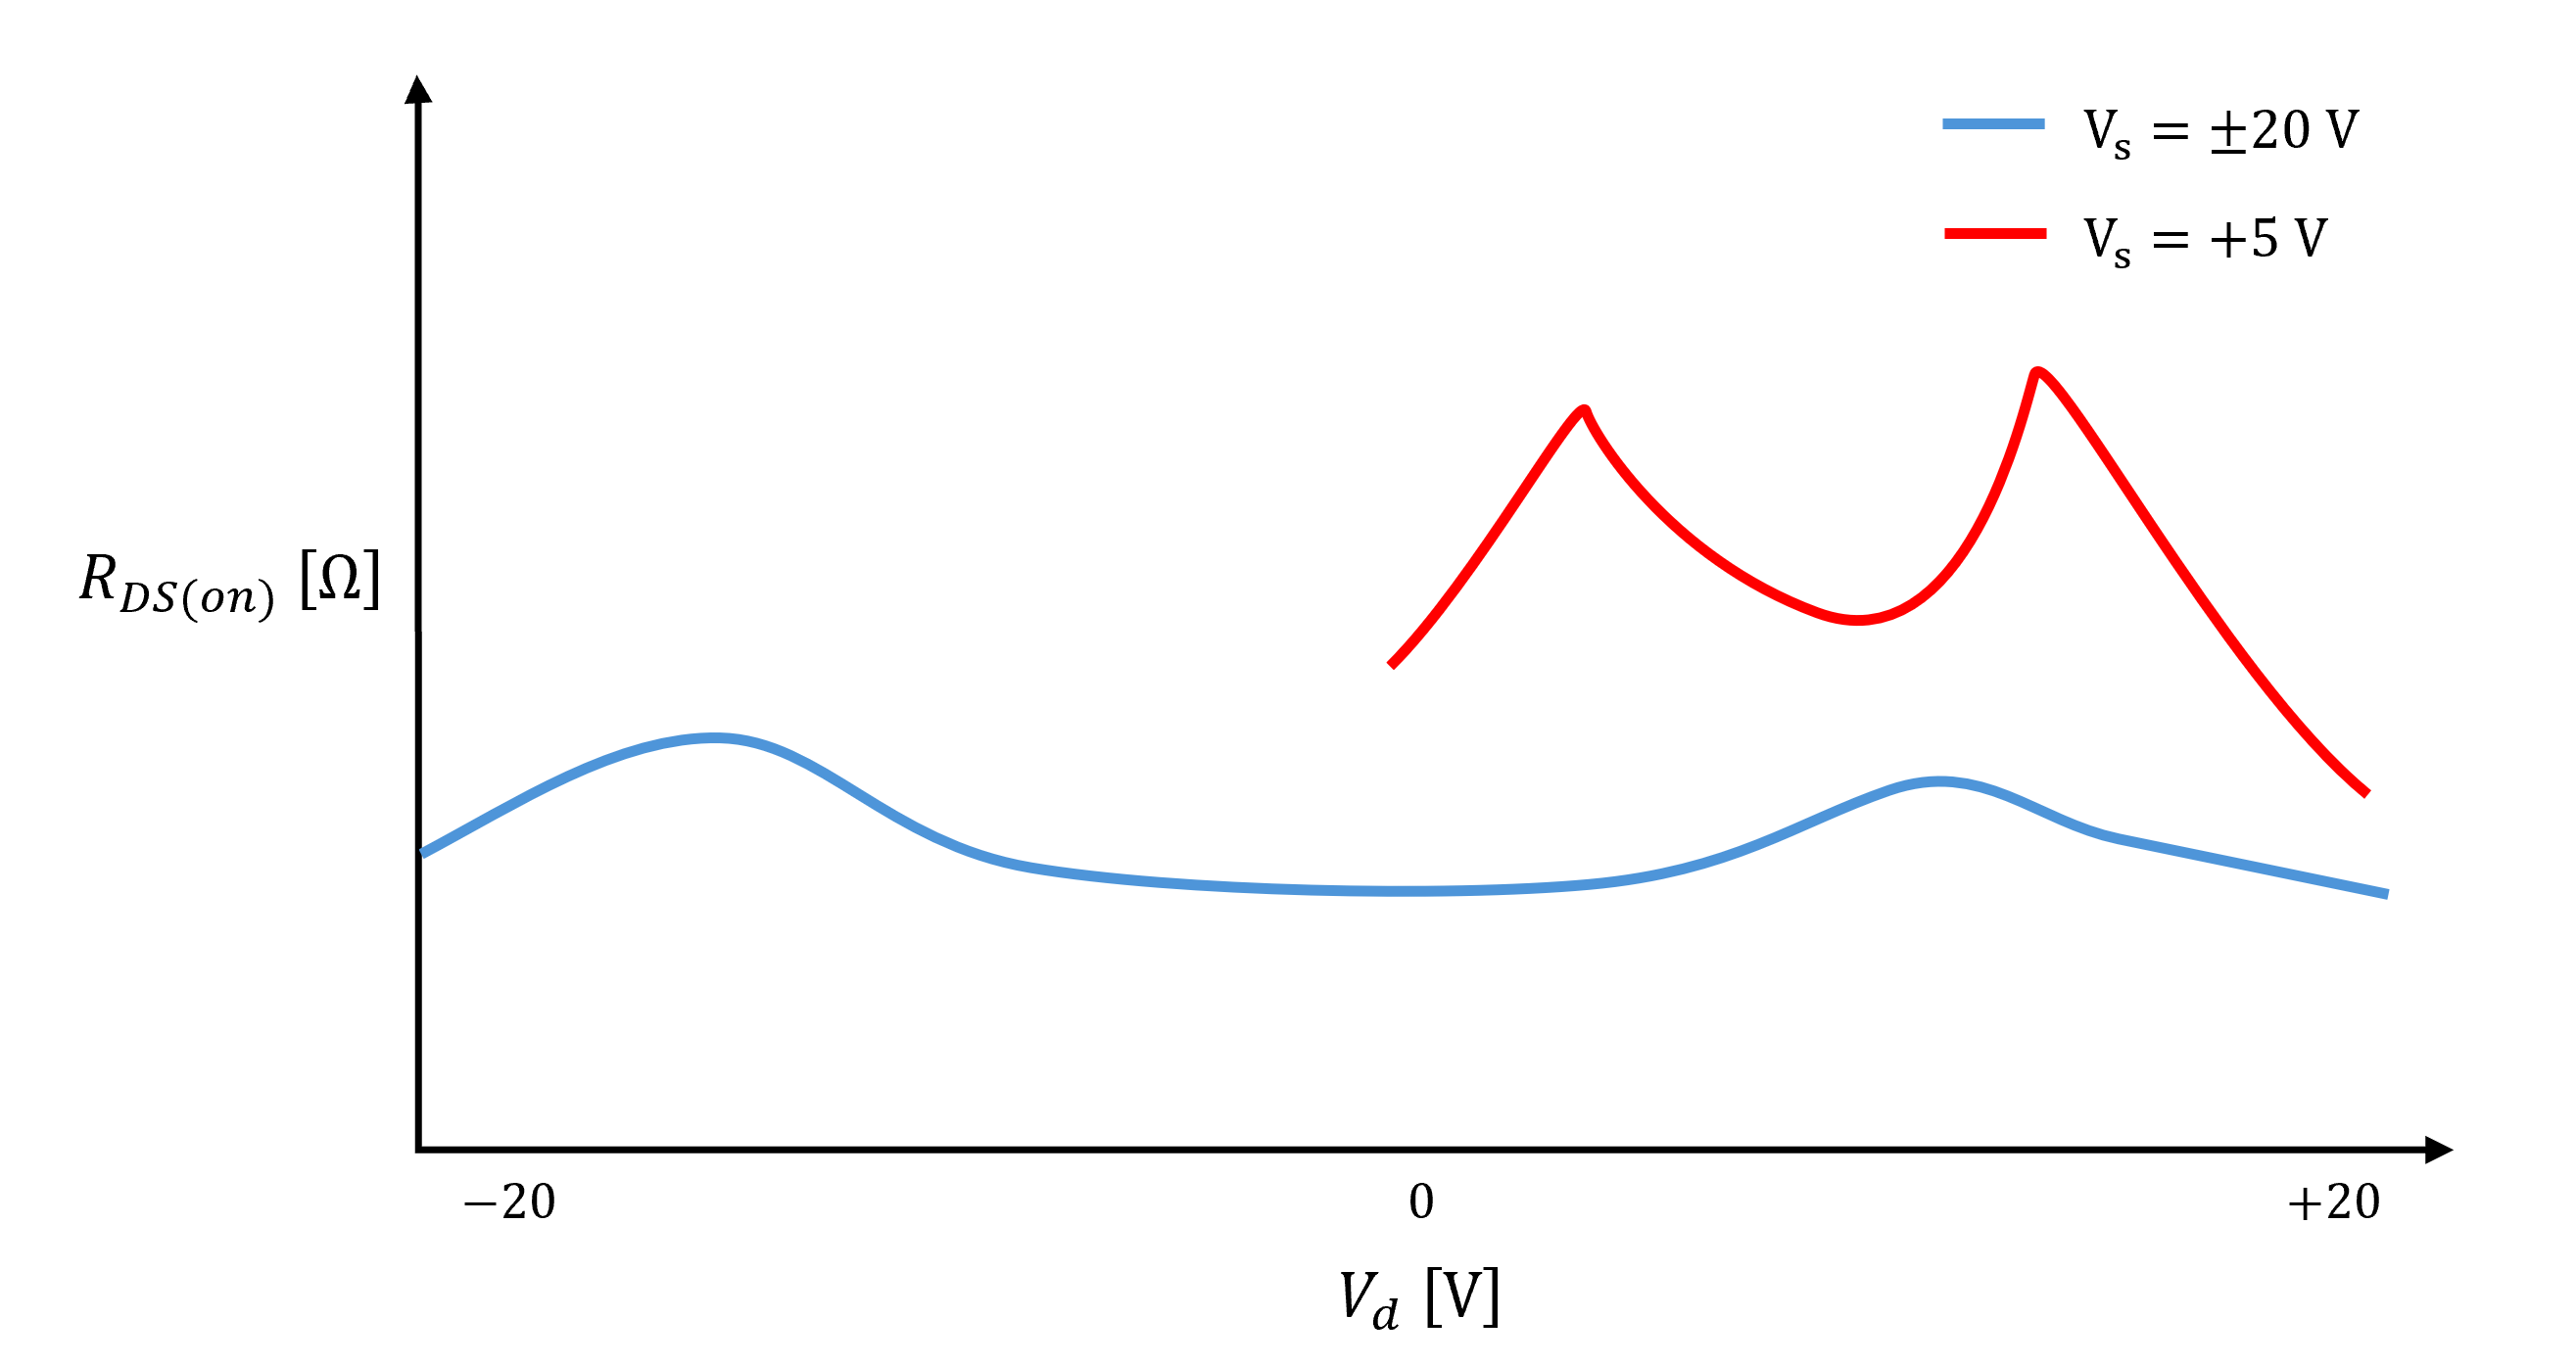
\includegraphics[width=0.6\linewidth]{Figures/mux_r_on_example.png}
\caption{$R_{DS(on)}$ characteristic diagram for a typical multiplexer analogue channel for a dual and single-ended power supply.}\cite{Vishay2024}.
\label{fig:mux_r_on}
\end{figure}

% >> redo this with actual analog switch p-mos n-mos device function. See \href{https://pdfserv.maximintegrated.com/en/an/AN5299.pdf}{AN5299.pdf}

Any variation in the $R_{DS(on)}$ value as a function of $V_D$ or from channel-to-channel will add to the offset noise read by the ADC lowering the resolution of the ERT pressure sensor. This low $R_{DS(on)}$ variation can be seen in Figure \ref{fig:mux_r_on}. The multiplexer used can switch analogue voltage up to $\pm$22 V with a switching time of 200 ns \cite{Vishay2024}.


\subsection{Force measurement}
The CFA system is designed to be used with soft piezoresistive sensing domains due to loading limitations of the 3D printer frame and the force applicator head design. The force applicator head must be significantly more rigid than the sensing domain being tested to ensure low strain error. 

A static load FEA simulation was completed on the loadcell bracket [PR9] with the maximum load expected used as 100N. The material of the bracket was PLA with orthotropic material properties. The static simulation used the orthotropic 3D printed PLA properties given by Sosa-Vivas et al. \cite{SosaVivas2023} with Caculix FEM solver \cite{Dhondt2023}. As shown in Figure \ref{fig:FEA_force_aplc} the maximum predicted displacement of an FEM element within the loadcell part was 0.13 mm. If using a sufficiently soft domain and small force applicator this maximum displacement has little effect on the data processed, however this may cause significant error within harder domains and/or larger force applicators. Although the device can operate at 100 N, device operation is recommended below 50 N to decrease the strain error due to force applicator deformation.

% TODO - redo FEA analysis

\begin{figure}[H]
\centering
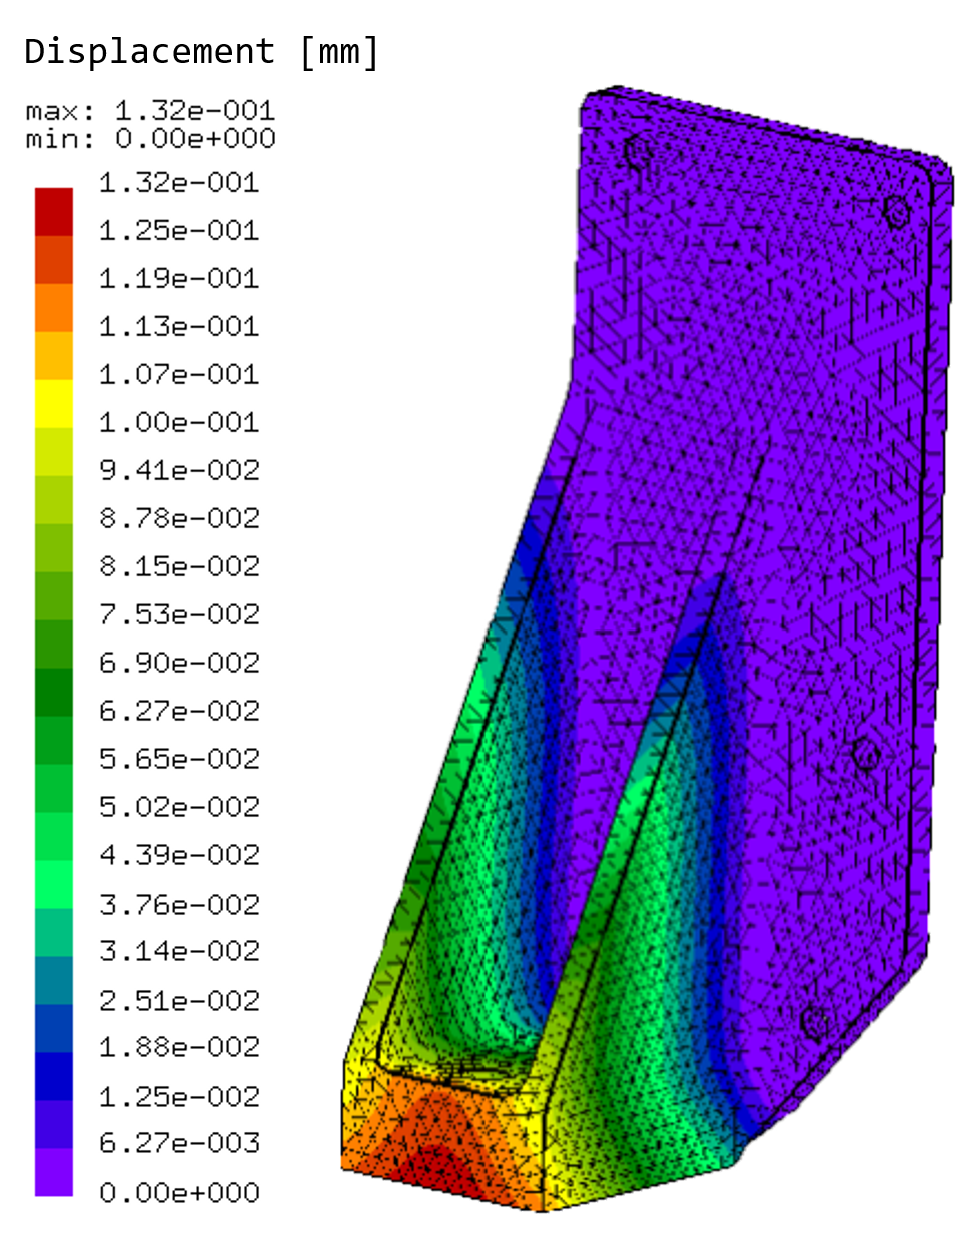
\includegraphics[width=0.4\linewidth]{Figures/fea_ccx_loadcell_bracket.png}
\caption{Static load analysis of the loadcell bracket part [PR9] of maximum allowable load of 100 N showing the magnitude of displacement. }
\label{fig:FEA_force_aplc}
\end{figure}

The TAL220 loadcell used was chosen for the sensing domain material. The CBSR material had an elastic modulus of 100 kPa\cite{Ellingham2024} so that range of strain measurements from 0 - 50\% could be accurately recorded with the given loadcell. The minimum force is on the limit of what can be detected as the TAL220 is rated for $\pm$50 mN resolution \cite{HTCSensor2024} across its operating load and temperature range. However the noise of the loadcell was measured to be $\pm$ 2.5 mN during several 15 minute experiments in a 22$\pm$0.7$\degree$C regulated room. Examples of experiment loading limits are given in Table \ref{tab:cfa_limits}, giving the extreme cases for testing minimum and maximum theoretical strain for 5 and 20 mm diameter force applicator heads on a lower and higher elastic modulus material respectively.
\begin{table}[H]
\caption{An example of the extreme parameters of two loading experiments showing the minimum and maximum strains limits for 5 mm and 20 mm diameter force applicators and their required forces respectively.}
\label{tab:cfa_limits}
\begin{tabular}{|p{1.8cm}|p{3.5cm}|p{3.5cm}|p{3.1cm}|p{2.1cm}|p{2.2cm}|} \hline
	\textbf{Force [N]} &
	\textbf{Force applicator diameter [mm]} &
	\textbf{Force applicator area [$\mathbf{mm^2}$]} &
	\textbf{domain elastic modulus [kPa]} &
	\textbf{Theoretical strain [\%]} &
	\textbf{Theoretical stress [kPa]} \\ \hline
	0.06 &
	5 &
	19.6 &
	60 &
	5.1 &
	3.1 \\ \hline
	50.00 &
	20 &
	314.2 &
	200 &
	79.6 &
	159.2 \\ \hline
\end{tabular}
\end{table}


% TODO: Calcs for the stepper motor strength

\subsection{Position control and measurement}
% justify position measurement system. Stepper motors don't skip and can step 0.XX mm increments? Serial-PC connection. Feed it array of strain magnitudes, locations, duration, and strain speed.
The Prusa MK3s 3D printer was used because of it's proven reliability as a 3D printer to move in x, y, and z axes with high resolution. The resolution of the force applicator location under without applying a load is 0.01 mm in each axis. Due to the open-loop nature of control of the stepper motors the resolution at high loads may not be reliable.

\subsection{Sensing domain}
% percolation etc. Mention recommended sonication bath usage.
The weight percentage of CB powder in an elastomer matrix, such as silicone rubber, to maintain desired mechanical and electrical properties can be tuned as shown in the characterisations completed by D'Asaro et al and Shang et al \cite{D'Asaro2017, Shang2016}. The most desirable piezoresistive characteristics found in these works are near the inflection point of the conductivity versus CB weight percentage plot.

Because of the difference in fabrication processes and degree of dispersion generating variability in the percolation, an iterative trial and error approach using the starting point found in literature was used to get 8 wt \% and 9 wt \% values for CB in SR \cite{D'Asaro2017, Shang2016}. Within this range the material was sufficiently conductive while maintaining mechanical strength through sufficient elastomeric cross-linking. Previous research indicates that there is a weight percentage at which the gauge-factor/piezoresistivity is at a maximum within a similar range used in this work \cite{Dong2017, Yang2020}. The CB particle dispersion can vary throughout a domain depending on various factors in the fabrication process including mixing technique, solvents used, silicone viscosity, particle size, particle agglomerations, amongst other factors \cite{Kalyon2002,Rodgers2010,Lux1993,Xu2016}. Dispersion of carbon black particles was ensured by using a relatively low viscosity silicone of 6,000 mPa.s and a centrifugal planetary mixer a method proven to give better dispersion than other traditional mixing techniques \cite{Thinky2010}.


\section{Operation instructions}
%Provide detailed instructions for the safe and proper operation of the hardware. 
%> Step-by-step operational instructions for operating the hardware. 
%> Use visual instructions as necessary. 
%> Highlight potential safety hazards.
To validate and characterise the ERT pressure mapping sensor the CFA is used to apply a sequence of loads to the material. The below sequence of required operations to complete this experiment includes: 
\begin{enumerate}
\item ERT sensor power modes
\item ERT sensor programming
\item ERT sensing domain preparation
\item Load application point and strain configuration
\item Touch based mesh bed leveling
\item Load experiment execution
\item Data capture
\item Data processing
\end{enumerate}
This sequence of events is repeated for different sensing domains and different loading conditions.

\subsection{ERT sensor power modes}
\label{sec:Operating modes}
Before running any experiments, the ERT sensor power mode must be configured. The jumper configuration for the bipolar supply (blue) and +5 V USB single-ended supply (red) mode is shown in Figure \ref{fig:ert_pcb_pinout_mode}.

The bipolar supply first mode is recommended for driving the ERT signal through a wider range of sensing domains at a higher voltage. A bipolar supply of $\pm$20 V is connected to $\pm V_s$ for the best performance of the circuit.

The second power mode uses a +5 V USB 3.X power supply to run the ERT circuit. The second mode is limited to lower resistance sensing domains that can be tested as it can only drive constant currents using +5 V. When using the +5 V supply mode the $-V_s$ and GND pins on the power input must be shorted for the multiplexers to operate. 
\begin{figure}[H]
\centering
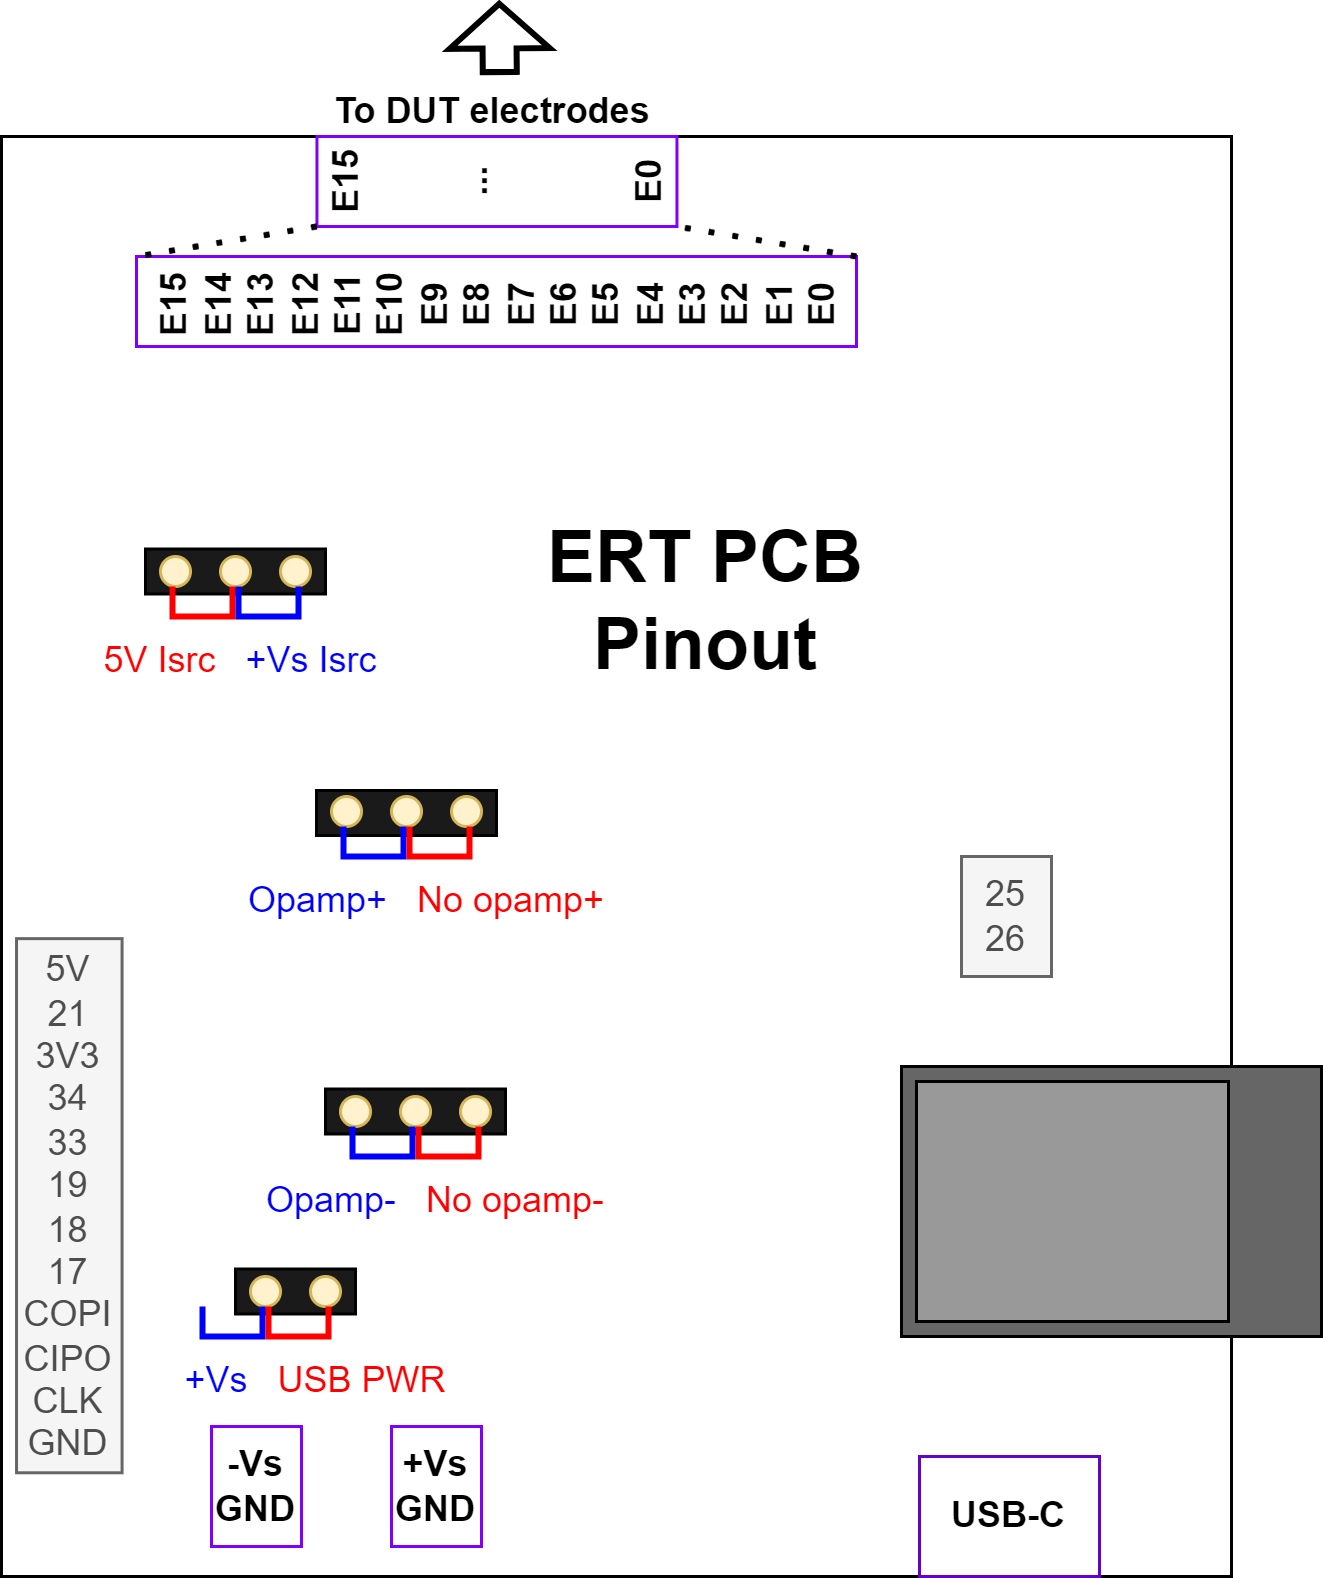
\includegraphics[width=0.3\linewidth]{Figures/ert_pcb_pinout.png}
\caption{ERT PCB pin-out and power mode options. Blue jumpers are for the bipolar supply mode (i.e. $\pm V_s$ attached). Red jumpers are for the +5 V USB supply mode. }
\label{fig:ert_pcb_pinout_mode}
\end{figure}
For each power mode there will be a distortion of the signal dependent on the power supply voltages and input signal as exemplified in Figure \ref{fig:mux_r_on}.


\subsection{ERT sensor programming}
The ERT sensor contains an ESP-WROOM32 module [U1] which requires the \verb|main_ert.c| program to be built and flashed. This can be achieved using the default project template from the \href{https://docs.espressif.com/projects/esp-idf/en/stable/esp32/get-started/index.html}{ESP-IDF environment}\cite{espressif2024}. The default ERT circuit firmware \verb|main_ert| completes the well proven adjacent electrode drive pattern \cite{Avis1992,Xu2008,Dang2021,Zamora-Arellano2020}. Upon successful programming of the ERT circuit it will output a constant serial stream of the adjacent electrode pattern ERT data separating each frame of 256 measurements with an `\verb|A|'. The ERT sensor circuit has the capability to send the real-time serial ERT data via a USB serial, Bluetooth, or WiFi connection to a EIT reconstruction capable computer.


\subsection{ERT sensing domain preparation}
For sensing domain fabrication instructions refer to Section \ref{sec:Sensing Domain}. The ERT sensing domain needs to have sufficiently low adjacent inter-electrode resistance to function, so that the current source will not saturate due the power supply voltage. The ET electrodes can be attached to the domain in many ways as shown in Figure \ref{fig:CBSR_samples_examples}, ensure these connections provide a reliable electrical contact to the sensing domain. Connect sensing domain electrodes to the ERT circuit FPC connector[W1] via an adapter[J8]. The ERT sensing domain must be flat and centered on the sensing domain holder [PR3, PR4] as shown in Figure \ref{fig:CBSR_samples_examples} (middle). 


\subsection{Load application point and strain configuration}
Load application points and strains applied to the sensing domain can be configured by altering variables in \verb|ertpcb_cfa_reader.py| code. A loading sequence consists of a series of load applications, in the form of a strain pulse train, applied to a set of X and Y coordinates on the sensing domain. The main parameters to change for running a loading sequence are given in Table \ref{tab:ert_cfa_params}.
\begin{table}[H]
\caption{Experimental parameters.}
\label{tab:ert_cfa_params}
\begin{tabu} to \linewidth {X[0.5,1] X[0.1,1] X}
	\textbf{Variable:}  & \textbf{Unit:} & \textbf{Description:} \\ \hline
	Strain speed (\texttt{v\_z\_push}) & mm/min & The rising/falling edge gradient for each pulse. \\
	Strain limit (\texttt{strain\_limit}) & \% & The maximum compressive strain allowed. \\
	Load locations (\texttt{push\_points}) & [mm, mm] & An array of XY locations of each load pulse. \\
	Reference offset (\texttt{ref\_loc\_mm}) & [mm, mm] & The XY offset of the zero point of the sensing domain relative to the CFA home reference. \\
\end{tabu}
\end{table}
% \begin{itemize}
%     \item Push time [s] - The time each strain pulse is held for.
%     \item Strain displacement speed [mm/min] - The rising/falling edge gradient for each pulse.
%     \item Load locations [mm, mm] - the xy locations of each load pulse.
%     \item Strain values [\%] - The strain values of each load pulse. 
%     \item Sample thickness [mm] - The sample domain thickness
%     \item Current source [A] - The constant current source value.
% \end{itemize}
These can all be found as variables in the software file \verb|ertpcb_cfa_reader.py| within the \verb|main| function. Before running this program the serial COM ports may need to be changed in the \verb|ertpcb_cfa_reader.py| program to match the comports of the CFA and ERT sensor hardware.

\subsection{Load experiment execution}
Once all hard-coded parameters have been set the command parameters are set and the load experiment begins. To begin the load experiment use the following terminal command:
\begin{verbatim}
>> python ertpcb_cfa_reader.py <dir/filename> <Isrc_A> <Vmax> <sample_name> <date_fabricated>
\end{verbatim}
\vspace{-1cm}
\begin{verbatim}
<load_time_s> <strain>
\end{verbatim}

Where \verb|<dir/filename>| is includes the file directory and file name, \verb|<Isrc_A>| is the constant current source value set in the ERT circuit in amps, \verb|<Vmax>| is the maximum allowed voltage to be read by the ADC in volts (e.g. 20 V), \verb|<sample_name>| is a descriptive sensing domain name, \verb|<date_fabricated>| is the sample fabrication date (`NA' or leave blank if irrelevant), \verb|<load_time_s>| is the strain pulse on and off time in seconds, and \verb|<strain>| is the desired strain applied to the domain as a percentage. If a random test sequence is desired with randomised strain and locations this can be achieved by simply setting the \verb|<strain>| value to -1.


\subsection{Touch-based mesh bed leveling}
% if sample isn't perfectly flat mesh bed leveling can compensate.
An undulating sensing domain surface can often be present during testing due to an intentionally curved sensor or manufacturing defects. To compensate for an uneven surface a touch-based mesh bed leveling process has been created to improve the quality of the stress/strain data gathered. The process involves the force applicator head travelling towards the sample until a change in force has been detected above 0.1 N. This mitigates the risk of any misalignment with the force applicator surface plane and the sensing domain surface plane and ensures more accurate strain data capture for low strain magnitudes. This touch-based mesh bed leveling is completed before the load sequence experiment begins. The sensing domain and holding trays should not be physically contacted in any form after beginning the \verb|ertpcb_cfa_reader.py| program.


\subsection{Data capture}
Once the \verb|ertpcb_cfa_reader.py| program has completed capturing data, a time-series plot of the 16 inter-electrode resistances, $R_{int}$, will appear. A stable $R_{int}$ is for stable EIT reconstructions of the sensing domain.  

Any significant change in the inter-electrode resistance may cause a poor EIT reconstruction result. A significant change in the inter-electrode resistance could be a result of, applying force too close to the electrodes themselves, an inherently unstable electrode connection, or an external force applied near the electrode. If the $R_{int}$ values are not stable it will be evident in the plot and there will be a warning message in the console. 
\begin{figure}[H]
\centering
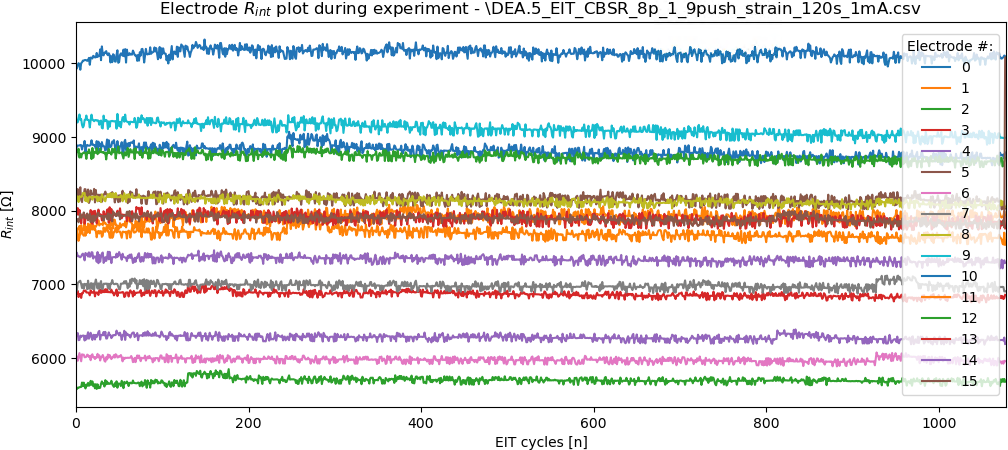
\includegraphics[width=0.75\linewidth]{Figures/Rint_plot.png}
\caption{An example plot of the $R_{int}$ values generated on completion of an experiment for a stable experiment. Where the Electrode \# `i' represents the resistance between electrode `i' and `i+1'.}
\label{fig:ert_pcb_pinout_mode}
\end{figure}
Once the inter-electrode resistance plot is closed the program will continue to save all of the data in three separate files for the given \verb|filename|,
\begin{enumerate}
\item \textit{filename}.csv - Time series data for ERT voltages, compression forces, and force applicator XYZ locations. The UTC start date and time of the experiment is given in the top row.  
\item \textit{filename}.pkl - Logs the same data as the .csv file \textbf{and} all of the important experiment parameters into a serialised python `pickle' file.
\item \textit{filename}.gcode - The gcode file of the commands sent to the 3D printer platform for the experiment run.
\end{enumerate}


\subsection{Data processing}
% Default EIT reconstruction algorithm (don't need to provide this)
Once all of the data has been collected in the above steps, the data can be processed. Data processing includes the following,
\begin{enumerate}
\item Pre-processing of the raw voltage, force, and position data. Filtering and data cleaning could be included in this step.
\item Image reconstruction using a chosen EIT algorithm with the pre-processing or raw data. EIT reconstruction could include algorithms such as regularised Newton's methods \cite{Lionheart2004}, neural network based methods \cite{Biasi2022, Husain2021}, and back projection methods \cite{Avis1992}.
\item Any post-processing of the EIT image reconstruction data and integration with the force applicator stress and/or strain data. Post-processing could include resistance to force inverse modelling, pressure mapping performance metric quantification, an application specific software interface.
\end{enumerate}
In this work EIDORS \cite{Sherry2006} has been used to complete the EIT reconstructions of the domain and any post processing is then completed with a python program as shown in Section \ref{sec:Validation and characterisation}.



\section{Construction and Operational Safety}
Various safety concerns must be stated for the construction and operation precautions of this system. This is not a comprehensive safety guide, but will give an overview of some potential safety concerns. Other precautions may be necessary depending on the development location and sensing domain materials used. The construction and operation of the system can each be separated into three parts, the ERT sensor circuit, the CFA, and the sensing domain.


\subsection{Construction}
During the assembly of the ERT sensor circuit the regular health and safety procedures for assembling and soldering a PCB must be followed.

During testing of the CFA as a 3D printer there will be moving parts which could get caught on long hair or collide with a person too close. Steps must be taken to avoid any undesired collisions or any people touching the CFA during operation.

When fabricating the sensing domain often this involves micro/nano sized conductive particles dangerous for inhalation and sometimes dangerous to touch. The material safety datasheet must be consulted for any material used in the sensing domain. Any safety procedures with mixing machines and curing devices must be followed.

\subsection{Operation}
The PCBA can operate on up to $\pm$ 20 VDC which is within the safe level the SELV as defined by IEC \cite{IEC2005}. However, should the contacts of the power supply to the ERT circuit be electrically shorted, a burn or fire hazard may arise. The current on the sensing domain electrodes is limited to prevent a dangerous short circuit current.

During the operation of the CFA there will be moving parts which could collide tangle long hair or collide with the person operating. Steps must be taken to avoid any undesired collisions or any people touching the CFA during operation.

The sensing domain may not be bio-compatible so the material safety datasheet(s) for each domain must be followed for each real world sensor application.


\section{Validation and characterisation}
\label{sec:Validation and characterisation}
%Demonstrate the operation of the hardware and characterize its performance over relevant critical metrics
%> Demonstrate the use of the hardware for a relevant use case. 
%> If possible, characterize performance of the hardware over operational parameters. 
%> Create a bulleted list that describes the capabilities (and limitations) of the hardware. For example consider descriptions of load, operation time, spin speed, coefficient of variation, accuracy, precision and etc.
To show that the system is functional, the plots produced from an EIT reconstruction of the voltage data and the force measurements can be compared for a correlation. Examples are given below in Figure \ref{fig:rand_recon_result} and \ref{fig:rand_recon_and force_result}, showing localised blobs at the known locations of the force applicator.
\begin{figure}[H]
\centering
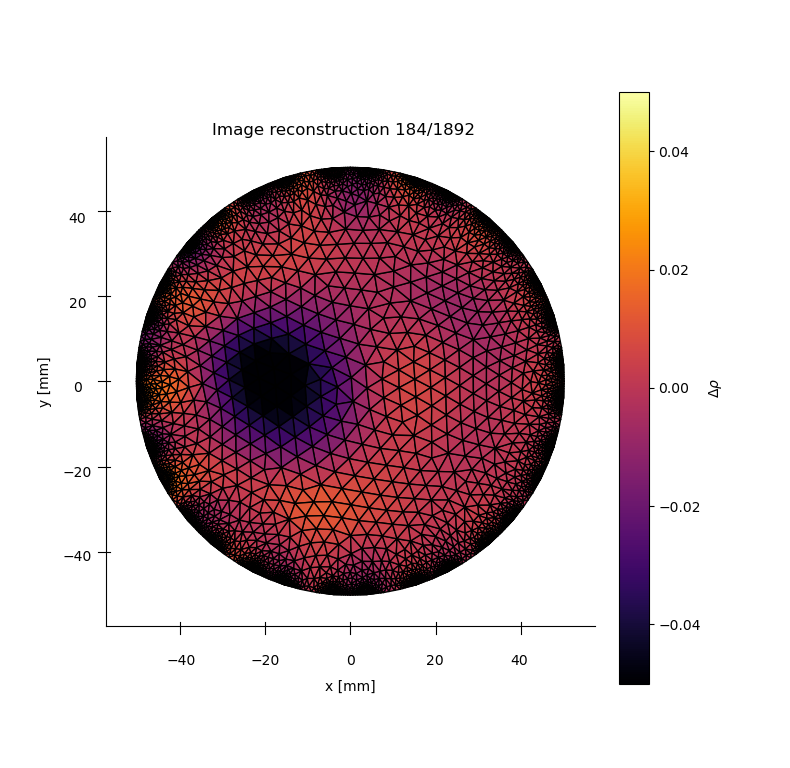
\includegraphics[width=0.45\linewidth]{Figures/DEA1_CBSR_8p_9push_rand10strain_30s_1mA_1_frame184.png}
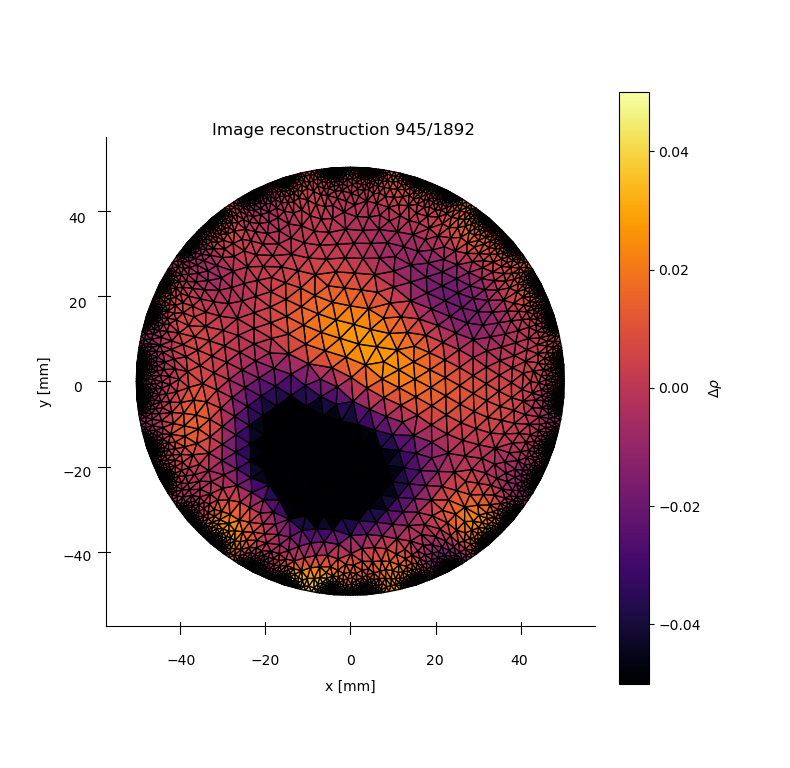
\includegraphics[width=0.45\linewidth]{Figures/DEA1_CBSR_8p_9push_rand10strain_30s_1mA_1_frame945.png}
\caption{Reconstruction frames from a random push test sequence on a 1mm thick 100mm diameter sample. Strain and applied locations (x, y) [mm] - Left: 24\% (-14.8, -3.4). Right: 36\% (-1.9, -21.3)}
\label{fig:rand_recon_result}
\end{figure}
A raw video of this experiment can be seen in the \verb|/examples| folder. It can be useful to plot the force profile being applied alongside the EIT reconstruction to verify the data is ready for further processing and modelling. 
\begin{figure}[H]
\centering
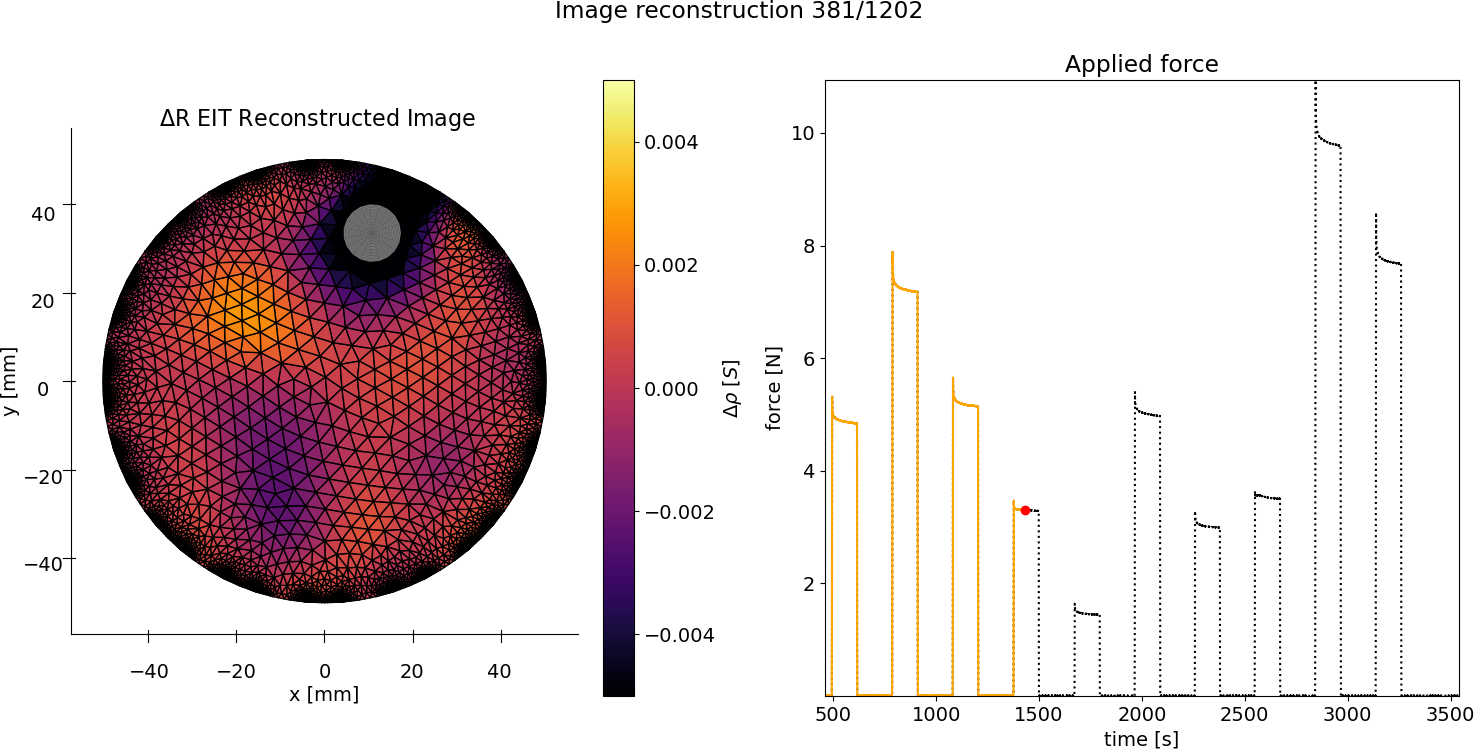
\includegraphics[width=\linewidth]{Figures/CBSR_8p_OG_10push_RAND1_strain_120s_1mA_2_frame381.png}
\caption{Reconstruction frames from a random push test sequence on a CBSR 100mm diameter sample. The white circle representing the force applicator location and the red dot on the force plot showing the captured frame in time.}
\label{fig:rand_recon_and force_result}
\end{figure}

% \subsection{Data collection rate}
% To ensure a range of load event durations can be detected and processed promptly a sufficiently high sample frequency is required.  
% votlage data averaging tradeoff?
% theoretical vs actual sample rate limit. What's the bottle neck? plots?
% USB serial vs Bluetooth vs Wifi

\subsection{Sensor capabilities}

Simultaneous application of multiple loads can be achieved with this system using a multi-head force applicator. It has been shown that multiple touch points can be detected as shown in Figure \ref{fig:multi-touch-eit} the supplementary material and in our previous work \cite{Ellingham2022}.
\begin{figure}[H]
\centering
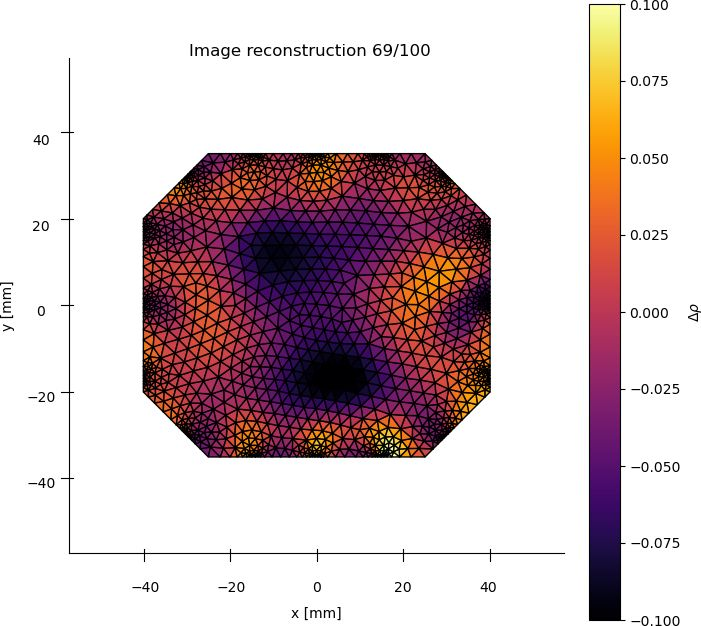
\includegraphics[width=0.4\linewidth]{Figures/multitouch_rect_CBSR_8p_80x70mm_frame69.jpg}% using 1.5mm thick 70 x 80 mm rectangle with 15 mm radius on corners
\hspace{1cm}
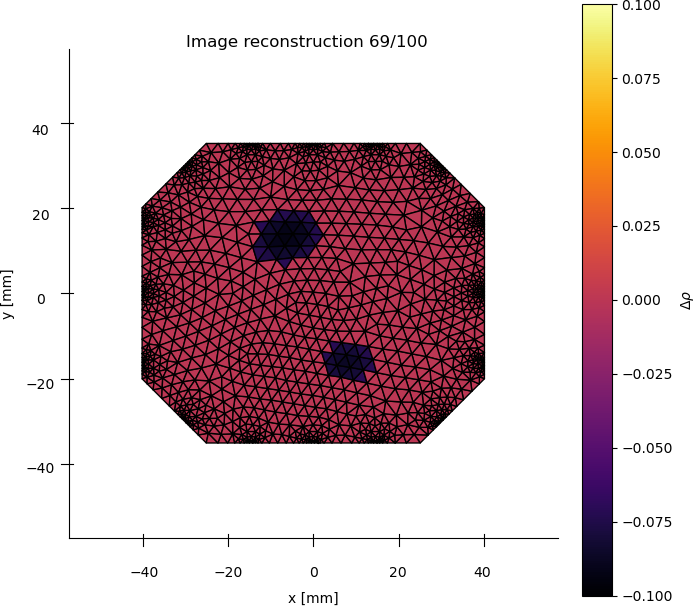
\includegraphics[width=0.4\linewidth]{Figures/multitouch_rect_CBSR_8p_80x70mm_frame69_75p_thresh.png}% using 1.5mm thick 70 x 80 mm rectangle with 15 mm radius on corners
\caption{An EIT reconstruction image of a sensing domain with two loads applied simultaneously. Left: Without threshold filtering. Right: With a 75\% threshold amplitude filter applied.}
\label{fig:multi-touch-eit}
\end{figure}

% >> currently sorting out new mesh for rectangular domain with filleted corners! :D

A major factor constraining the application of EIT-based sensors is the poor frequency response of the material, which limits the detection of rapid successive loads. The system given in this work allows further research into characterising the transient response of a range of sensing domains in 2D. Examples of how transients have been characterised are shown in Figure \ref{fig:2D-transient}
\begin{figure}[H]
\centering
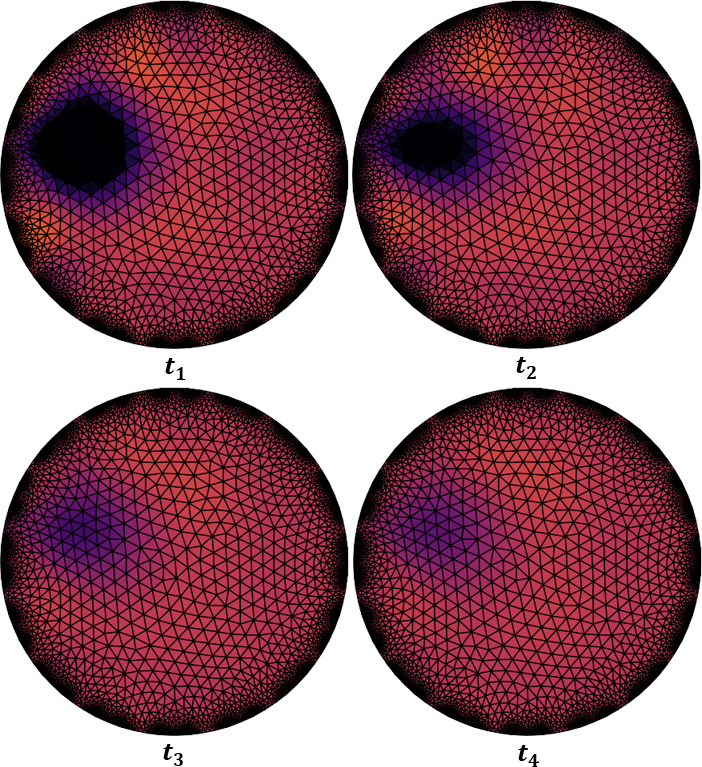
\includegraphics[width=0.3\linewidth]{Figures/res_relax_DEA_EIT_1mm_3load_7kV_1.png}
\hspace{1cm}
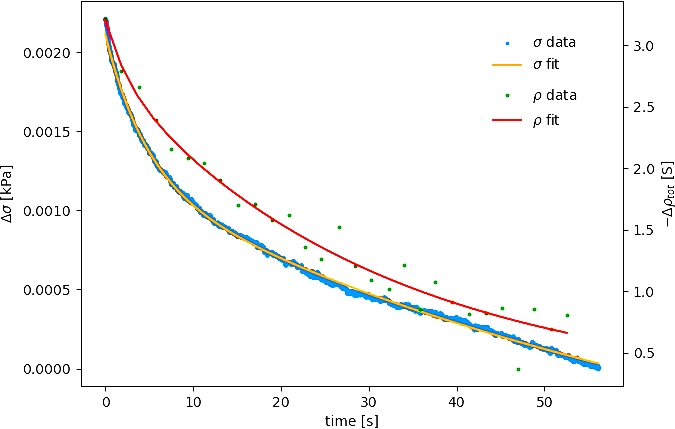
\includegraphics[width=0.5\linewidth]{Figures/2D Push event 0 - CBSR 9 wt 30p strain - 2D compressionv2.jpg}
\caption{Left: Example sequence a resistive relaxation after a loading event at times $t_1$ to $t_4$. Right: Example stress, $\sigma$, and resistive, $\rho$, relaxation plot generated from an ERT CFA experiment given a 30\% strain step input \cite{Ellingham2024}.}
\label{fig:2D-transient}
\end{figure}

The piezoresistivity of a sensing domain can often vary throughout its volume giving unpredictable results if a homogeneous domain is assumed for the pressure mapping sensor. This system can be used to generate map of the piezoresistivity function of a material surface in 2D dimensions.

% Any non-ideal conditions in the data measurement process affect the EIT reconstruction quality. Several factors affect the data gathered from the system including, temperature, humidity, component variation, electrode noise, power supply noise, ERT circuit component defects, externally generated mechanical vibrations, and ambient electrical noise \cite{?,?,?,?}. 

% >> Could just remove the above paragraph??

% \subsection{Sensitivity Analysis}
% To quantify how robust the system will be over a range of input noise values a range of noise values are added to the system and the resulting noise factors are determined.

\section{Conclusions}
This work has provided the methods and tools to enable further research and development for soft EIT-based pressure sensing systems. The system is low cost, simple to construct, and easy to use. The automation of compression load experiments ensures that experiments are repeatable with quantifiable results and mitigating human error. The automated nature of the CFA device significantly reduces the time to complete a set of experiments and can provide experiment sequences similar to those expected during the real-world application of the sensor. Upon load experiment completion, the system provides clearly formatted raw data files ready for analysis.

% Current limitations of the system include: lack of closed loop feedback to ensure positional accuracy, the inherently jerky motion of stepper motors, the loadcell resolution for very soft loads, the software interface is could be more user friendly.

Uses of this system vary from 2D piezoresistive material analysis and pressure mapping sensor characterisation. Extensive research has been conducted into one-dimensional (1D) characterisation of piezoresistive materials. However, the characterisation of these materials in two dimensions (2D) has often been overlooked in past literature \cite{Ding2007,Shang2016,Buketov2020,Zhao2013}, often due to the complex and invasive methods required. The device can be used to characterise the electromechanical/piezoresistive properties of a soft thick film material in 2D, quantify EIT reconstruction performance, and generate models predicting localised loads from localised resistance changes.

To push the field of EIT-based pressure mapping forward tools are required to standardise testing and reliably acquire quantifiable data for pressure modelling in different sensing domain materials. A toolbox of hardware and software have been described in this work to make EIT-based pressure mapping realisable for more real-world applications.

Proposed future enhancements of the system include minimising noise and offsets in the signal conditioning ERT circuit, adding an auto-calibration procedure to ensure the ADC and $I_{src}$ circuits operate at the expected resolution, and reducing the PCB size. 
% ... picture of the vision for future applications ...
The ERT sensor and Cartesian force applicator system described in this work will help transition this technology into real-world applications.

\section{Future Work}
The integration of DEA and EIT in a portable package would open a range of applications. To integrate this portable EIT system into the DEA-EIT device mentioned in Chapters 6 and 7, a DEA driver expansion board would be required. This would give an DEA-EIT device could have the capability of contracting and acquiring EIT voltage data for pressure mapping while maintaining a small form factor. A draft design of the DEA PCBA mounted on the portable EIT PCBA can be seen in Figure \ref{fig:DEA-EIT_draft_pcb_assy}. 
\begin{figure}[H]
	\centering
	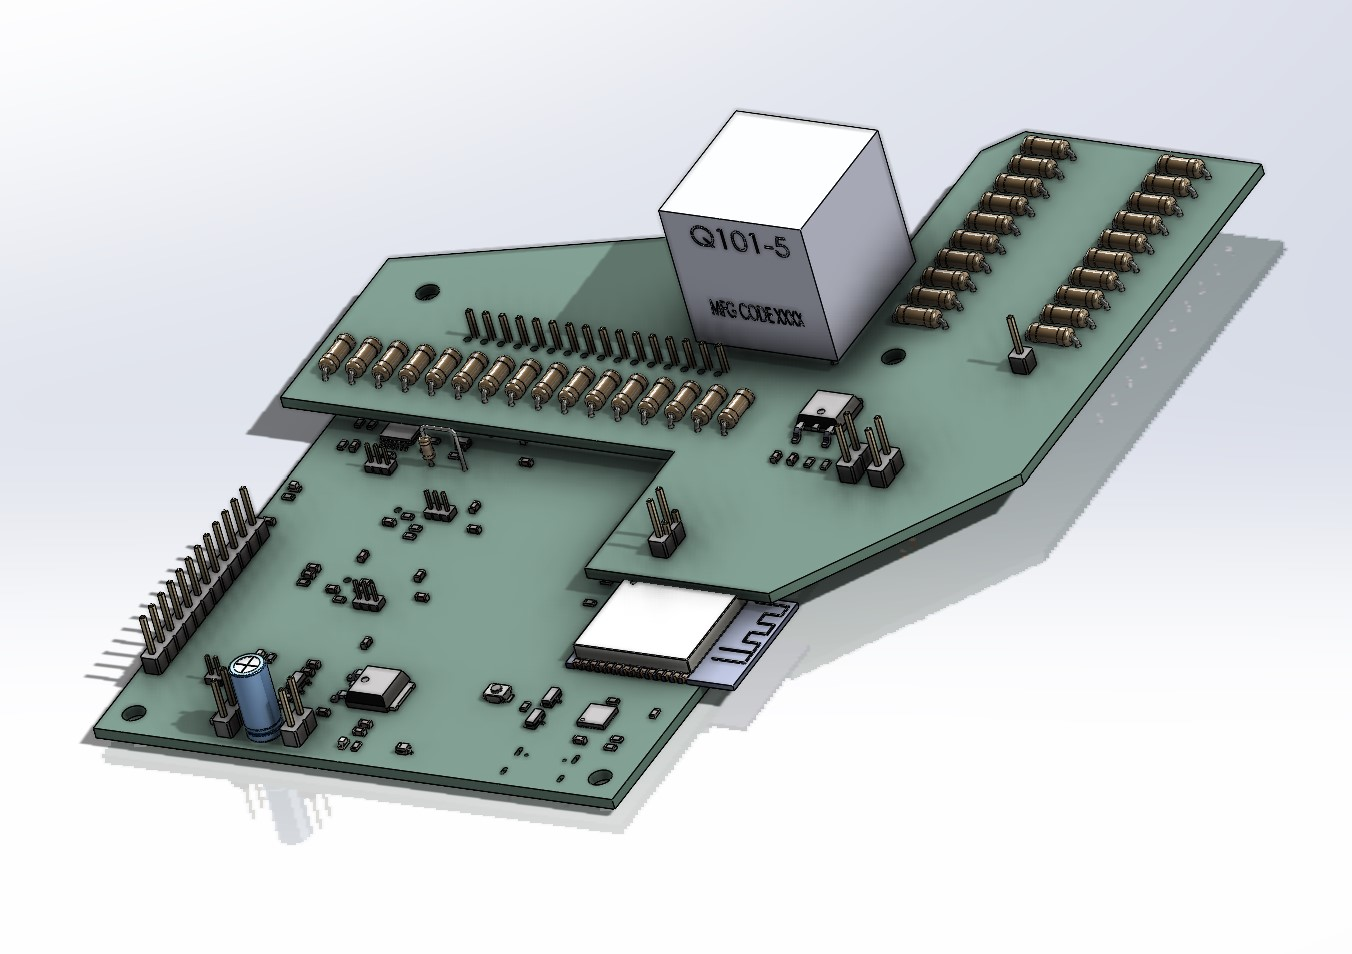
\includegraphics[width=0.55\linewidth]{Figures/DEA-EIT_mother-daughter_board_draft.jpg}
	\caption{Render of a DEA daughter board mounted on this work's portable ERT board.}
	\label{fig:DEA-EIT_draft_pcb_assy}
\end{figure}